%% \begin{subsection}{Overview}

The Slater-ISA methodology for short-range intermolecular interactions has
been derived from a simple but rigorous physical model of overlapping
monomer electron densities. In practice, this approach differs from the
conventional Born-Mayer approach in both the choice of the short-range
functional form (with the latter omitting the polynomial pre-factor) and the
source of the exponents (with the former derived from ISA analysis of the
monomer density). Our principal goal is to examine the influence of these
modifications on the accuracy and transferability of the resulting force
fields.

We initially benchmark the \isaffold against a conventional Born-Mayer potential,
\saptff.
%, where the -IP suffix denotes the fact that the atomic exponents $B_i$ have
%been derived from the isolated atomic ionization potentials.  
The latter approach has been used extensively in prior
work,\cite{Schmidt2015,McDaniel2013} and both approaches use identical numbers of
fitted parameters.  Following prior work, combination rules for the \saptff are as in
\citen{McDaniel2013}. (We have tested the effect of using a geometric mean
for the \saptff; results do not differ qualitatively from those presented
below.) Owing to its popularity, we also compare the \isaffold to a Lennard-Jones
functional form (\ljff).

We first assess the accuracy of the \isaffold, \saptff, and \ljff against benchmark
ab initio intermolecular interaction energies and experimental 2\super{nd}
virial coefficients, enthalpies of vaporization, and liquid densities. 
We next examine parameter transferability, assessing the
extent to which parameters from pure homo-monomeric systems can be re-used
(without further optimization) to describe mixed interactions. To assess 
parameter robustness, we also study the sensitivity of each methodology to
changes in the weighting function (\cref{eq:isotropic-weighting-function}). Finally, we
explore the application of \bsisa-derived exponents within the Born-Mayer
functional form as a straightforward method for simplifying the
parameterization (and potentially increasing the accuracy) of a wide variety of
standard ab initio and empirically-parameterized force fields.


\begin{subsection}{Accuracy: Comparison with DFT-SAPT}

For each of the 91 molecule pairs described in the \nameref{sec:isotropic-methods} section, 
parameters for the \isaffold, \saptff, and \ljff
were fit to reproduce \saptpbeo interaction energies calculated for a set of 1000 dimer
configurations. These 91,000 total configurations and corresponding DFT-SAPT
energies are collectively referred to as the `91 dimer test set'.  As a
primary indication of accuracy, root-mean-square errors (RMSE) and mean signed
errors (MSE), both with respect to DFT-SAPT, were computed for each
methodology and for each dimer pair. Because these RMSE and MSE are dominated by
repulsive contributions, and owing to the thermodynamic importance of
attractive configurations, so-called `attractive RMSE/MSE' were also computed by
excluding net repulsive configurations (as measured by the DFT-SAPT total energy). 
The overall RMSE/MSE for all 91 dimers were then
averaged to produce one `characteristic RMSE/MSE' for the entire test set.  Since
these errors varied considerably in magnitude depending on the dimer in
question, this overall average was taken in the geometric mean sense. (Results
with an arithmetic mean do not differ qualitatively). Note that when computing
the characteristic MSE, only the magnitude of each MSE, \mse, was considered.

Characteristic RMSE and \mse across the 91 dimer test set are shown in \cref{fig:isotropic-rmse}
and \cref{tab:isotropic-rmse}.  Overall, the \isaffold exhibits smaller errors compared
to the \saptff. On average, the characteristic total energy RMSE for the \isaffold
decrease by 33\% relative to the \saptff.  Even excluding repulsive configurations
(dominated by short-range interactions), errors for the \isaffold are lower by 11\%
compared to the \saptff, demonstrating modest gains in accuracy even over the most
energetically-relevant regions of the potential.  
A more detailed analysis of each of the 91 pairs of molecules shows that in an
overwhelming 93\% of such cases, force fields
derived from the Slater-ISA method have smaller RMSEs compared to their
Born-Mayer-IP counterparts (70\% if only attractive configurations are
considered). Regardless of the metric used, the \isaffold produces force
fields with higher fidelity to the underlying benchmark interaction energies.

    %%%%%%%%%%%% Average RMSE %%%%%%%%%%%%%%%
    \begin{figure}
    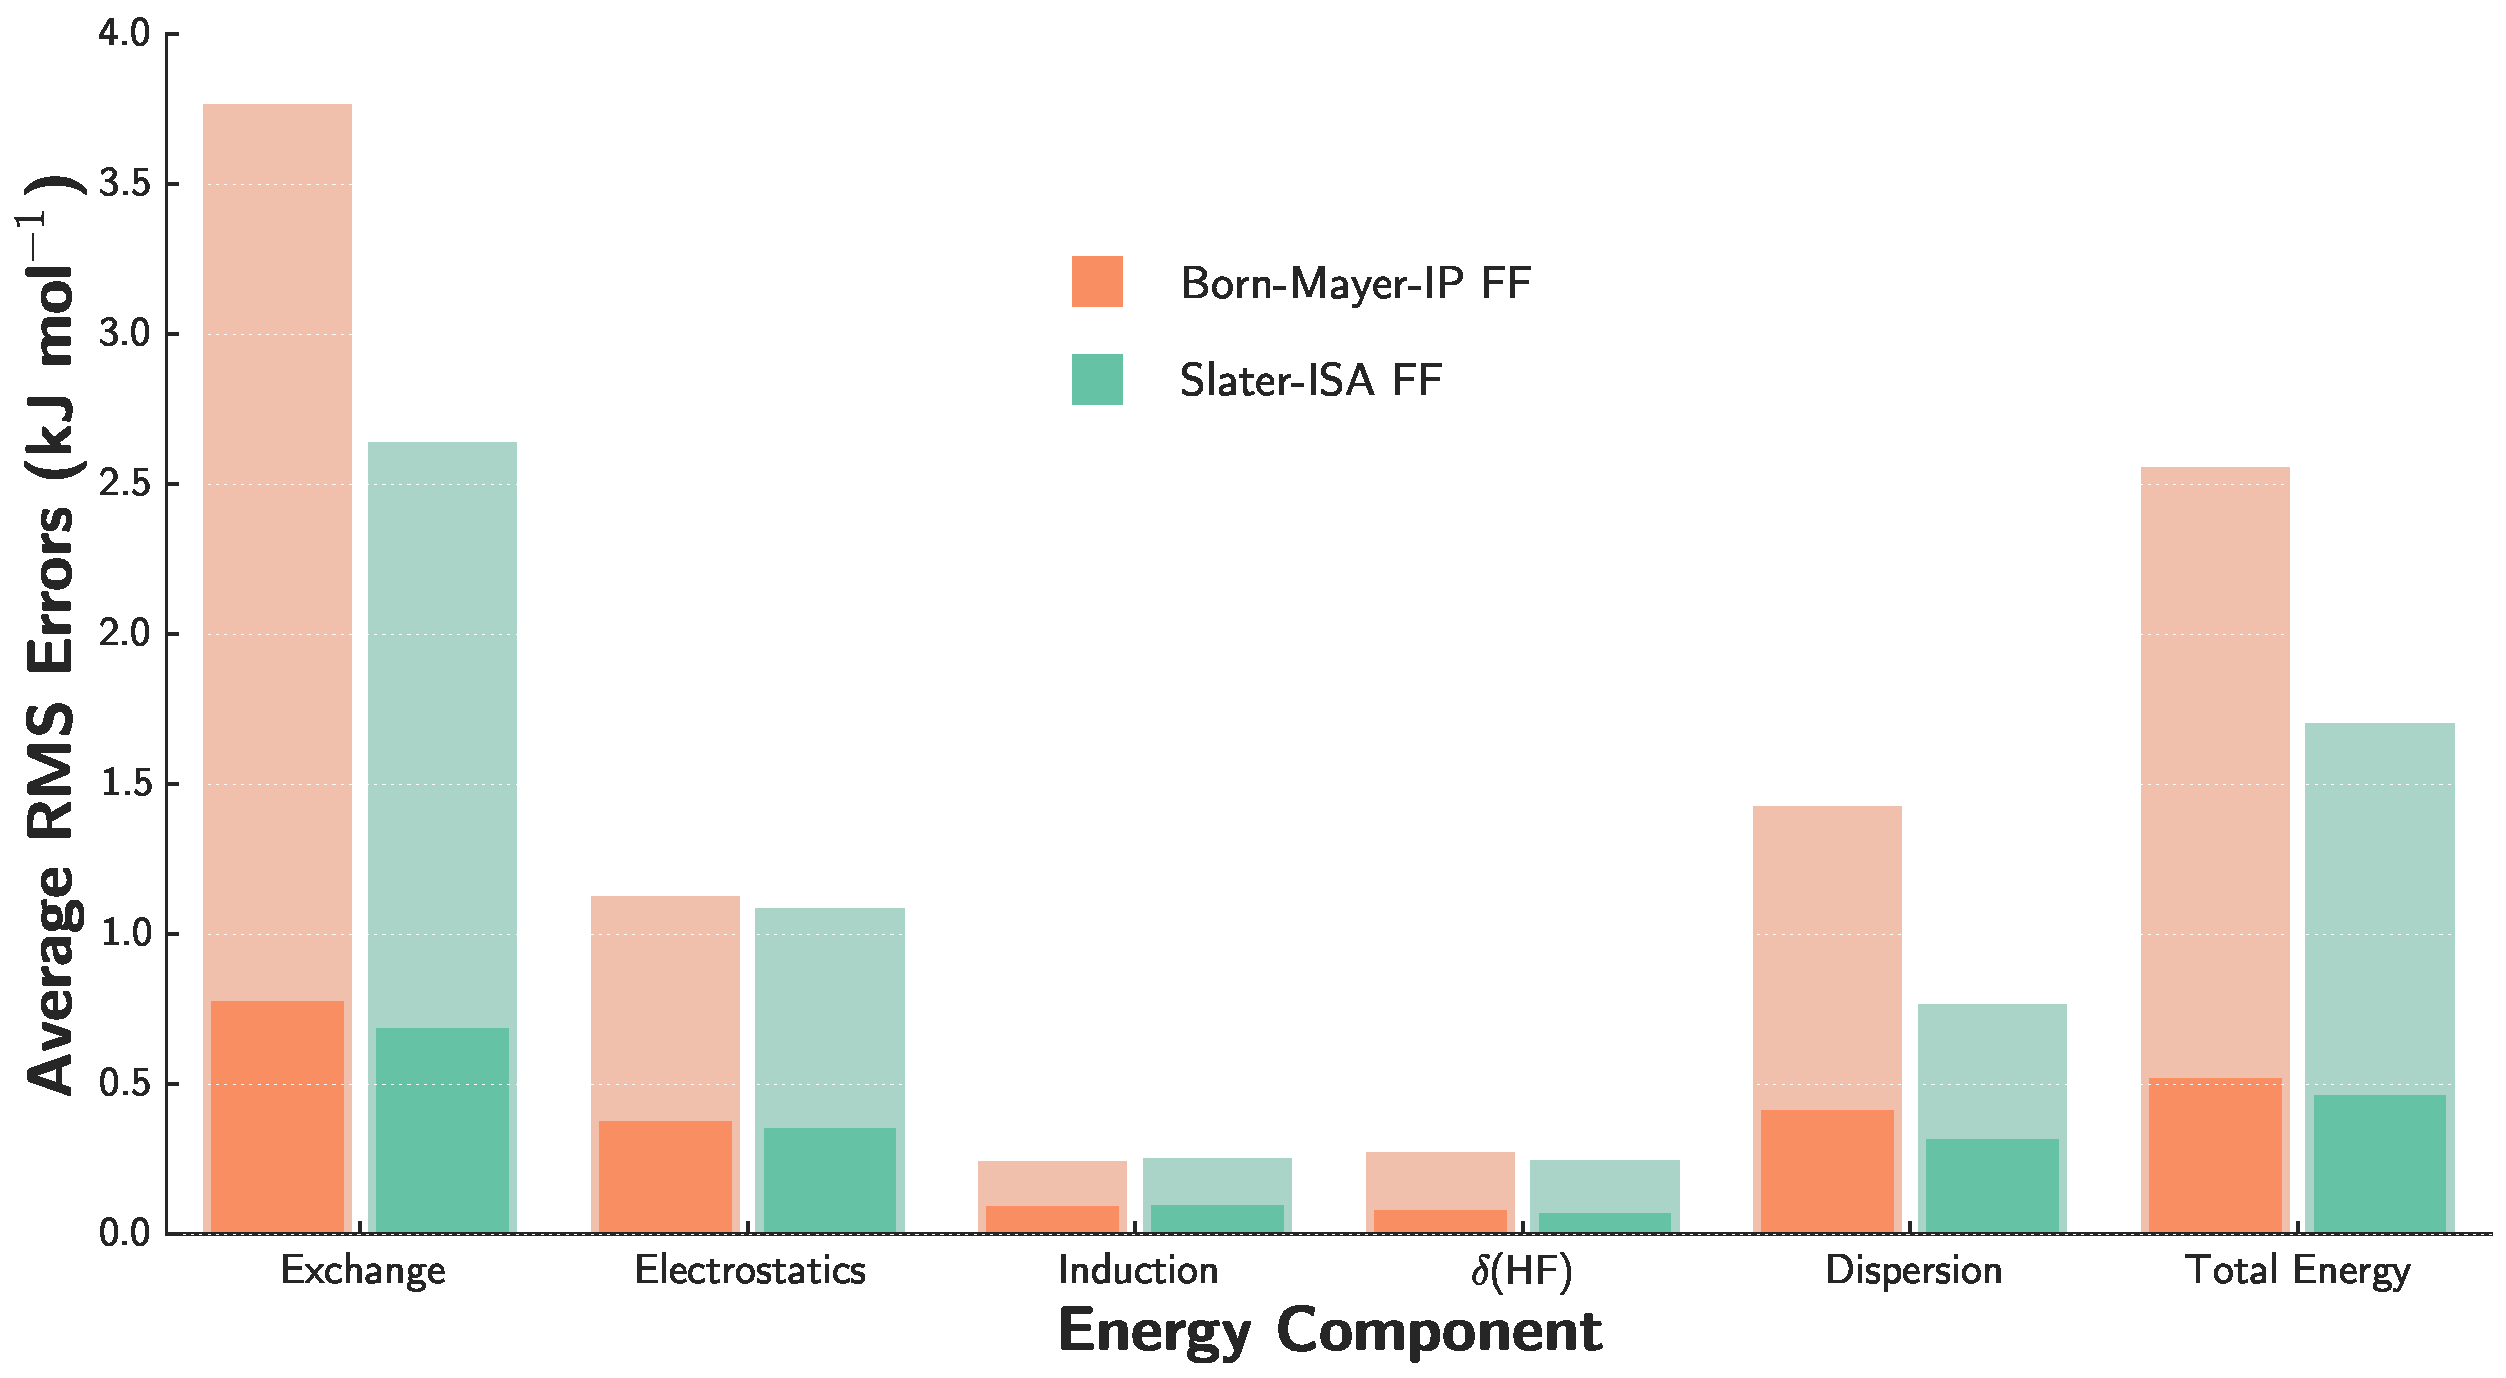
\includegraphics[width=0.9\textwidth]{isotropic/rmse_errors.pdf}
    \caption{
    Characteristic RMSE (as described in the main text) for the \saptff (orange) and the \isaffold (green) over the 91
    dimer test set. The translucent bars represent total RMSE
    for each energy component, while the smaller solid bars represent `Attractive'
    RMSE, in which repulsive points have been excluded.
            }
    \label{fig:isotropic-rmse}
    \end{figure}
    %%%%%%%%%%%% Average RMSE %%%%%%%%%%%%%%%

%%%%%%%%%%%%%%%%%%%%% Average RMSE Table %%%%%%%%%%%%%%%%%%%%%%%%%%%%%%%%%%%
\begin{landscape}
\begin{table}
\footnotesize
\centering
\renewcommand\arraystretch{1.1}
\begin{tabular}{@{}rcccccccc@{}}
\hline
\toprule
& \phantom{} &
  \multicolumn{3}{c}{Dimer-Specific Fits} &
  \phantom{ab} &
  \multicolumn{3}{c}{Transferable Fits} \\
\cmidrule{3-5} \cmidrule{7-9}

Component & & \isaffold & \saptff & \ljff & & \isaffold & \saptff & \ljff \\
     & & \multicolumn{1}{c}{(kJ mol$^{-1}$)} & \multicolumn{1}{c}{(kJ mol$^{-1}$)} &  \multicolumn{1}{c}{(kJ mol$^{-1}$)}
     & & \multicolumn{1}{c}{(kJ mol$^{-1}$)}& \multicolumn{1}{c}{(kJ mol$^{-1}$)} &  \multicolumn{1}{c}{(kJ mol$^{-1}$)}\\
\midrule
Exchange        & &    2.641 (0.686)   &    3.766 (0.775)   &     ---          & &    2.718 (0.720)  &    4.033 (0.836)   &     ---        \\
Electrostatics  & &    1.087 (0.351)   &    1.126 (0.377)   &     ---          & &    1.134 (0.351)  &    1.231 (0.378)   &     ---        \\
Induction       & &    0.251 (0.095)   &    0.241 (0.093)   &     ---          & &    0.278 (0.101)  &    0.265 (0.098)   &     ---        \\
\dhf            & &    0.246 (0.068)   &    0.272 (0.079)   &     ---          & &    0.274 (0.076)  &    0.304 (0.081)   &     ---        \\
Dispersion      & &    0.766 (0.317)   &    1.425 (0.414)   &     ---          & &    0.766 (0.317)  &    1.425 (0.414)   &     ---        \\
\addlinespace
\textbf{
Total Energy}  \\
\emph{RMSE}     & &    1.701 (0.464)   &    2.554 (0.520)   &   1.984 (0.603)  & &    1.650 (0.456)  &    2.698 (0.555)   &  2.054 (0.640) \\
%\addlinespace
%Average Absolute MSE    
\emph{\mse}
                & &    0.216 (0.057)   &    0.539 (0.127)   &    0.322 (0.345) & &    0.175 (0.051)  &    0.569 (0.112)  &    0.311 (0.368) \\
\bottomrule
\hline
\end{tabular}
\caption{
    Comparison of characteristic RMSE (as described in the main text) over the 91 dimer test
set for the \isaffold, \saptff and \ljff.
For the total energy, both characteristic RMSE and MSE have been shown, with
only the magnitude of the MSE, \mse, displayed.
    `Attractive' RMSE, representing the characteristic RMSE for
    the subset of points whose energies are net attractive ($\etot <
    0$), are shown in parentheses to the right of the total RMS
    errors; `attractive' \mse are likewise displayed for the total
    energy.
As discussed in \cref{ss:transferability}, the `Dimer-Specific Fits'
refer to force fields whose parameters have been optimized for each of the 91
dimers separately, whereas the `Transferable Fits' refer
to force fields whose parameters have been optimized for the 13 homodimers and
then applied (without further optimization) to the remaining 78 mixed systems.
    Unless otherwise stated, a default weighting function of $\lambda=2.0$
    (see \cref{eq:isotropic-weighting-function}) has been used for all force fields in
    this Chapter.
	}
\label{tab:isotropic-rmse}
\end{table}
\normalsize
\end{landscape}
%%%%%%%%%%%%%%%%%%%%% Average RMSE Table %%%%%%%%%%%%%%%%%%%%%%%%%%%%%%%%%%%

It is also instructive to consider each energy component individually.  As
might be expected, improvements in the description of \erep are pronounced,
with the characteristic RMSE from the \isaffold being 30\% smaller than that from the \saptff.
Examining each dimer pair separately (see
\cref{sec:isotropic-homomonomeric_fits} for homo-monomeric
fits, representative of the entire test set) we also find that, in general, the \isaffold
is far better at reproducing \emph{trends} in the exchange energy compared to
the \saptff. This qualitative result is also reflected in the smaller \mse
values for the \isaffold as compared to the \saptff.
Nevertheless, there remains a fair amount of scatter in the exchange
energies for several dimer pairs, particularly for molecules with exposed lone
pairs or delocalized $\pi$ systems. We hypothesize that this scatter is due to
a breakdown of the isotropic approximation made in the \nameref{sec:isotropic-theory}
section, a conclusion supported by observations on the pyridine dimer system
recently made by some of us.\cite{Misquitta2015b}
It it therefore quite possible that the observed 30\% RMSE reduction 
underestimates the true error reduction that might be observed
if such anisotropy were accounted for.

From  \cref{fig:isotropic-rmse}, we see that the dispersion energy model from the 
\isaffold is also a substantial improvement; for dispersion, characteristic RMSE
are 46\% smaller for the \isaffold compared to the Born-Mayer model.
This should not be a counter-intuitive result: while both potentials use identical
dispersion coefficients, they differ in the damping model used.
In the \saptff, the standard Tang--Toennies damping model is employed, and 
the damping parameters only depend on free atom ionization potentials; 
in the \isaffold, on the other hand, the damping parameters are obtained from the
ISA shape functions, and thus take 
molecular environment effects into account.
Even when only considering attractive dimer configurations (solid bar in
\cref{fig:isotropic-rmse}), errors in the dispersion energy component are reduced by 23\%,
demonstrating the importance of the damping function across the potential surface. 
From these results, and in agreement with related literature
studies,\cite{Sebetci2010} we conclude that use of
the standard Tang-Toennies damping function based on atomic ionization
potentials
\cite{Tang1984, Misquitta2008a, Price2010, Totton2010a, McDaniel2013, Hermida-Ramon2000, Nyeland1990} 
lacks quantitative predictive power compared to the Slater-ISA model.
Note that neither the \isaffold nor the \saptff are directly fitted to the DFT-SAPT
dispersion energies (all parameters are determined from monomer properties),
making this accuracy particularly striking.  We hypothesize that the effect of
the Slater-ISA approach is greater for dispersion than for first-order exchange
because here (in contrast to the exchange energy) there are no fitted
parameters to compensate for deficiencies in the exponents or functional form
of the \saptff.

In contrast to the exchange and dispersion energies, the \isaffold and the \saptff show nearly identical errors for the
electrostatic and the induction (2\super{nd} order induction plus \dhf) energies.
In these cases, the two models differ only in the parameters and functional form used to represent
the exponentially-dependent short-range terms of these energy components, 
namely the penetration component for the electrostatic term and the 
penetration/charge-transfer term for the induction.
The lack of improvement between the Slater-ISA and Born-Mayer-IP models may
imply that we are not 
able to capture the physics of these particular short-range interactions with
either the Slater-functional of Born-Mayer functional forms.
Alternatively, the assumption that the short-range components of the electrostatic 
and induction energies are proportional to the exchange-repulsion may need to be 
re-examined. As discussed in \cref{sec:isotropic-heteroatomic_vsr},
this proportionality is known to be approximately valid, but as yet there does 
not seem to be a deeper theoretical understanding of these short-range terms
that may lead to a better model.
Nevertheless, absolute errors in the electrostatic and induction components are
relatively small for both models.  Thus overall, the \isaffold functional form
is promising for treating a wide variety of short-range effects. 


%%%%%%%%%%%%%%%%%%%%% Average LJ RMSE Table %%%%%%%%%%%%%%%%%%%%%%%%%%%%%%%%%%%
%\begin{landscape}
\begin{table}
\footnotesize
\centering
\renewcommand\arraystretch{1.1}
\begin{tabular}{@{}rcccccc@{}}
\hline
\toprule
& \phantom{} &
  \multicolumn{2}{c}{\ljff Dimer-Specific Fits} &
  \phantom{ab} &
  \multicolumn{2}{c}{\ljff Transferable Fits} \\
\cmidrule{3-4} \cmidrule{6-7}

%% Component & & \ljff-q0, $\lambda=0.1$ & \ljff-q2, $\lambda=0.1$ & \ljff-q2, $\lambda=2.0$ 
%%           & & \ljff-q0, $\lambda=0.1$ & \ljff-q2, $\lambda=0.1$ & \ljff-q2, $\lambda=2.0$ \\

%%           & & \ljff               & \ljff             %  & \ljff-q0,               
%%           & & \ljff               & \ljff       \\    %  & \ljff-q0,               \\
          & &           $\lambda=2.0$ &           $\lambda=0.1$      %     $\lambda=0.1$ 
          & &           $\lambda=2.0$ &           $\lambda=0.1$   \\ %     $\lambda=0.1$ \\
     & & \multicolumn{1}{c}{(kJ mol$^{-1}$)} & \multicolumn{1}{c}{(kJ mol$^{-1}$)} % &  \multicolumn{1}{c}{(kJ mol$^{-1}$)}
     & & \multicolumn{1}{c}{(kJ mol$^{-1}$)}& \multicolumn{1}{c}{(kJ mol$^{-1}$)}  \\ % &&  \multicolumn{1}{c}{(kJ mol$^{-1}$)}\\
\midrule
%% RMSE             & &  1.984 (0.603)   &  6.058 (0.413)  &  5.116 (0.560)   && 2.054 (0.640)  &  5.760 (0.457)  &  4.513 (0.658) \\
%% Absolute MSE
%%                  & &  0.322 (0.345)   &  1.610 (0.041)  &  0.803 (0.038)   && 0.311 (0.368)  &  1.410 (0.060)  &  0.562 (0.079) \\
\emph{RMSE}             & &  1.984 (0.603)   &  6.058 (0.413)  && 2.054 (0.640)  &  5.760 (0.457)    \\
\emph{\mse}
                 & &  0.322 (0.345)   &  1.610 (0.041)  && 0.311 (0.368)  &  1.410 (0.060)    \\
\bottomrule
\hline
\end{tabular}
\caption{
    Comparison of characteristic RMSE and \mse over the 91 dimer test
set for the various Lennard-Jones models. The LJ models are not parameterized
on a component-by-component basis, thus RMSE/\mse values are only
shown for the total FF energies.
    `Attractive' errors, representing the characteristic RMSE/\mse for
    the subset of points whose energies are net attractive ($\etot <
    0$), are shown in parentheses to the right of the total 
    errors. `Dimer-Specific Fits' and `Transferable Fits' are as in \cref{tab:isotropic-rmse}.
	}
\label{tab:isotropic-lj_rmse}
\end{table}
\normalsize
%\end{landscape}
%%%%%%%%%%%%%%%%%%%%% Average LJ RMSE Table %%%%%%%%%%%%%%%%%%%%%%%%%%%%%%%%%%%


The comparison between the \isaffold and the \ljff is slightly more complicated,
owing to the differences in long-range potential and fitting methodology (see
\cref{sec:isotropic-FF-forms}). As such, we compare the \isaffold to several versions of the
\ljff (for which characteristic RMSE and \mse are shown in 
\cref{tab:isotropic-lj_rmse}). Using the same weighting function and
constraining the Coulombic and polarization terms to be identical to the
\isaffold, we see that the resulting Lennard-Jones force field (\ljff,
$\lambda=2.0$) is significantly worse than the \isaffold, both in terms of total
RMSE and attractive RMSE. Furthermore, by comparing the \mse
of both force fields, we see that errors in
\ljff are much more \emph{systematic} than in the \isaffold: in order to
reproduce the repulsive wall correctly, the Lennard-Jones potential
generally underestimates the well-depth by a considerable fraction (see
the Supporting Information of \citen{VanVleet2016} for ethane as a typical example). 

Given the failure of the \ljff ($\lambda=2.0$) force field to reproduce the
energetically important region of the PES, we also compared the \isaffold to a
`best-case' scenario Lennard-Jones force field which correctly
reproduces the minimum energy region at the expense of the repulsive wall. These
\ljff ($\lambda=0.1$) fits have total RMSE errors nearly 4 times that of the
\isaffold; indeed, the \ljff ($\lambda=0.1$) reproduces the repulsive wall only
qualitatively. Insofar as the repulsive wall is concerned, the \isaffold is far
superior to the Lennard-Jones short-range model. Nevertheless (and much more
importantly for molecular simulation), the attractive region of the potential
is reproduced surprisingly well by \ljff. Characteristic attractive RMSE for
the \ljff ($\lambda=0.1$) are slightly lower than those for \isaffold, although
the former has one additional free parameter per atom type and is also fit directly
to reproduce the total energy. Likewise, attractive \mse between the
\isaffold and the \ljff ($\lambda=0.1$) are comparable. As we show in the
Supporting Information of \citen{VanVleet2016},
however, and as is well known in the literature, weighting the Lennard-Jones potential in this
manner does not necessarily capture important information from the long-range attractive tail or repulsive wall of the PES, such
that the \ljff ($\lambda=0.1$) is not always expected to yield good
property predictions. This latter point will be demonstrated in 
\cref{sec:isotropic-accuracy_experiment}.

In order to compare the performance of the \isaffold against popular standard
force fields, we also developed a `best case scenario' non-polarizable point
charge Lennard-Jones model, results for which are shown in the Supporting
Information of \citen{VanVleet2016}. Unsurprisingly, this force field is worse (in an
RMSE and \mse sense) than all
other force fields studied in this Chapter, thus demonstrating how important
accurate models for long-range electrostatics and polarization are to the
overall accuracy of ab initio force fields.

\begin{subsubsection}{Argon Dimer}

We now turn to several specific case studies. The Ar dimer provides an interesting test
case to examine directly the impact of the polynomial pre-factor included in
the \isaffold functional form. 
Since Ar is an atomic species, we should have $\Bisa{\text{Ar}} = \Bip{\text{Ar}}$.
For numerical reasons, the \isaffold and \saptff exponents differ by 0.03 a.u.;
however, this difference is insignificant, and the two FFs differ mainly in the
polynomial pre-factor.
\cref{fig:isotropic-ar-pes} shows the potential energy
surface (PES) for the argon dimer computed using the \isaffold and the \saptff.
Here the default weighting scheme has been used so as to best reproduce the energetically
attractive region. Note that, while both potentials reproduce the minimum energy
configurations correctly, the \saptff considerably overestimates the exchange energy (and thus
the total energy) along the repulsive wall.
The \isaffold, on the other hand, maintains excellent accuracy in this region of the
potential. This result is particularly notable because the repulsive wall is not heavily weighted in the fit.
(A point 10 kJ mol$^{-1}$ along the repulsive wall, for instance, is weighted only 3\% as
heavily as a point near the bottom of the well).
A similar, though smaller, increase in accuracy is seen in the fit to the
DFT-SAPT dispersion energies, where the \isaffold is better able to model the
energies for shorter interatomic separations.  This increased accuracy is
entirely attributable to the functional form employed, as the dispersion
parameters are identical between the two FFs.

Consistent with prior literature,\cite{Ihm1990, McDaniel2012} these results
suggest that neglect of the polynomial pre-factor $P$ (as in standard
Born-Mayer potentials) is \emph{by itself} a poor approximation. However, as
we show below, the Born-Mayer form can still be used as an accurate model
in conjunction with appropriately scaled atomic exponents. Nonetheless, the
more physically-motivated Slater form provides increased accuracy over a wider
range of separations without recourse to empirical scaling.


    %%%%%%%%%%%% Ar-Ar PES %%%%%%%%%%%%%%%%%%
    \begin{figure}
    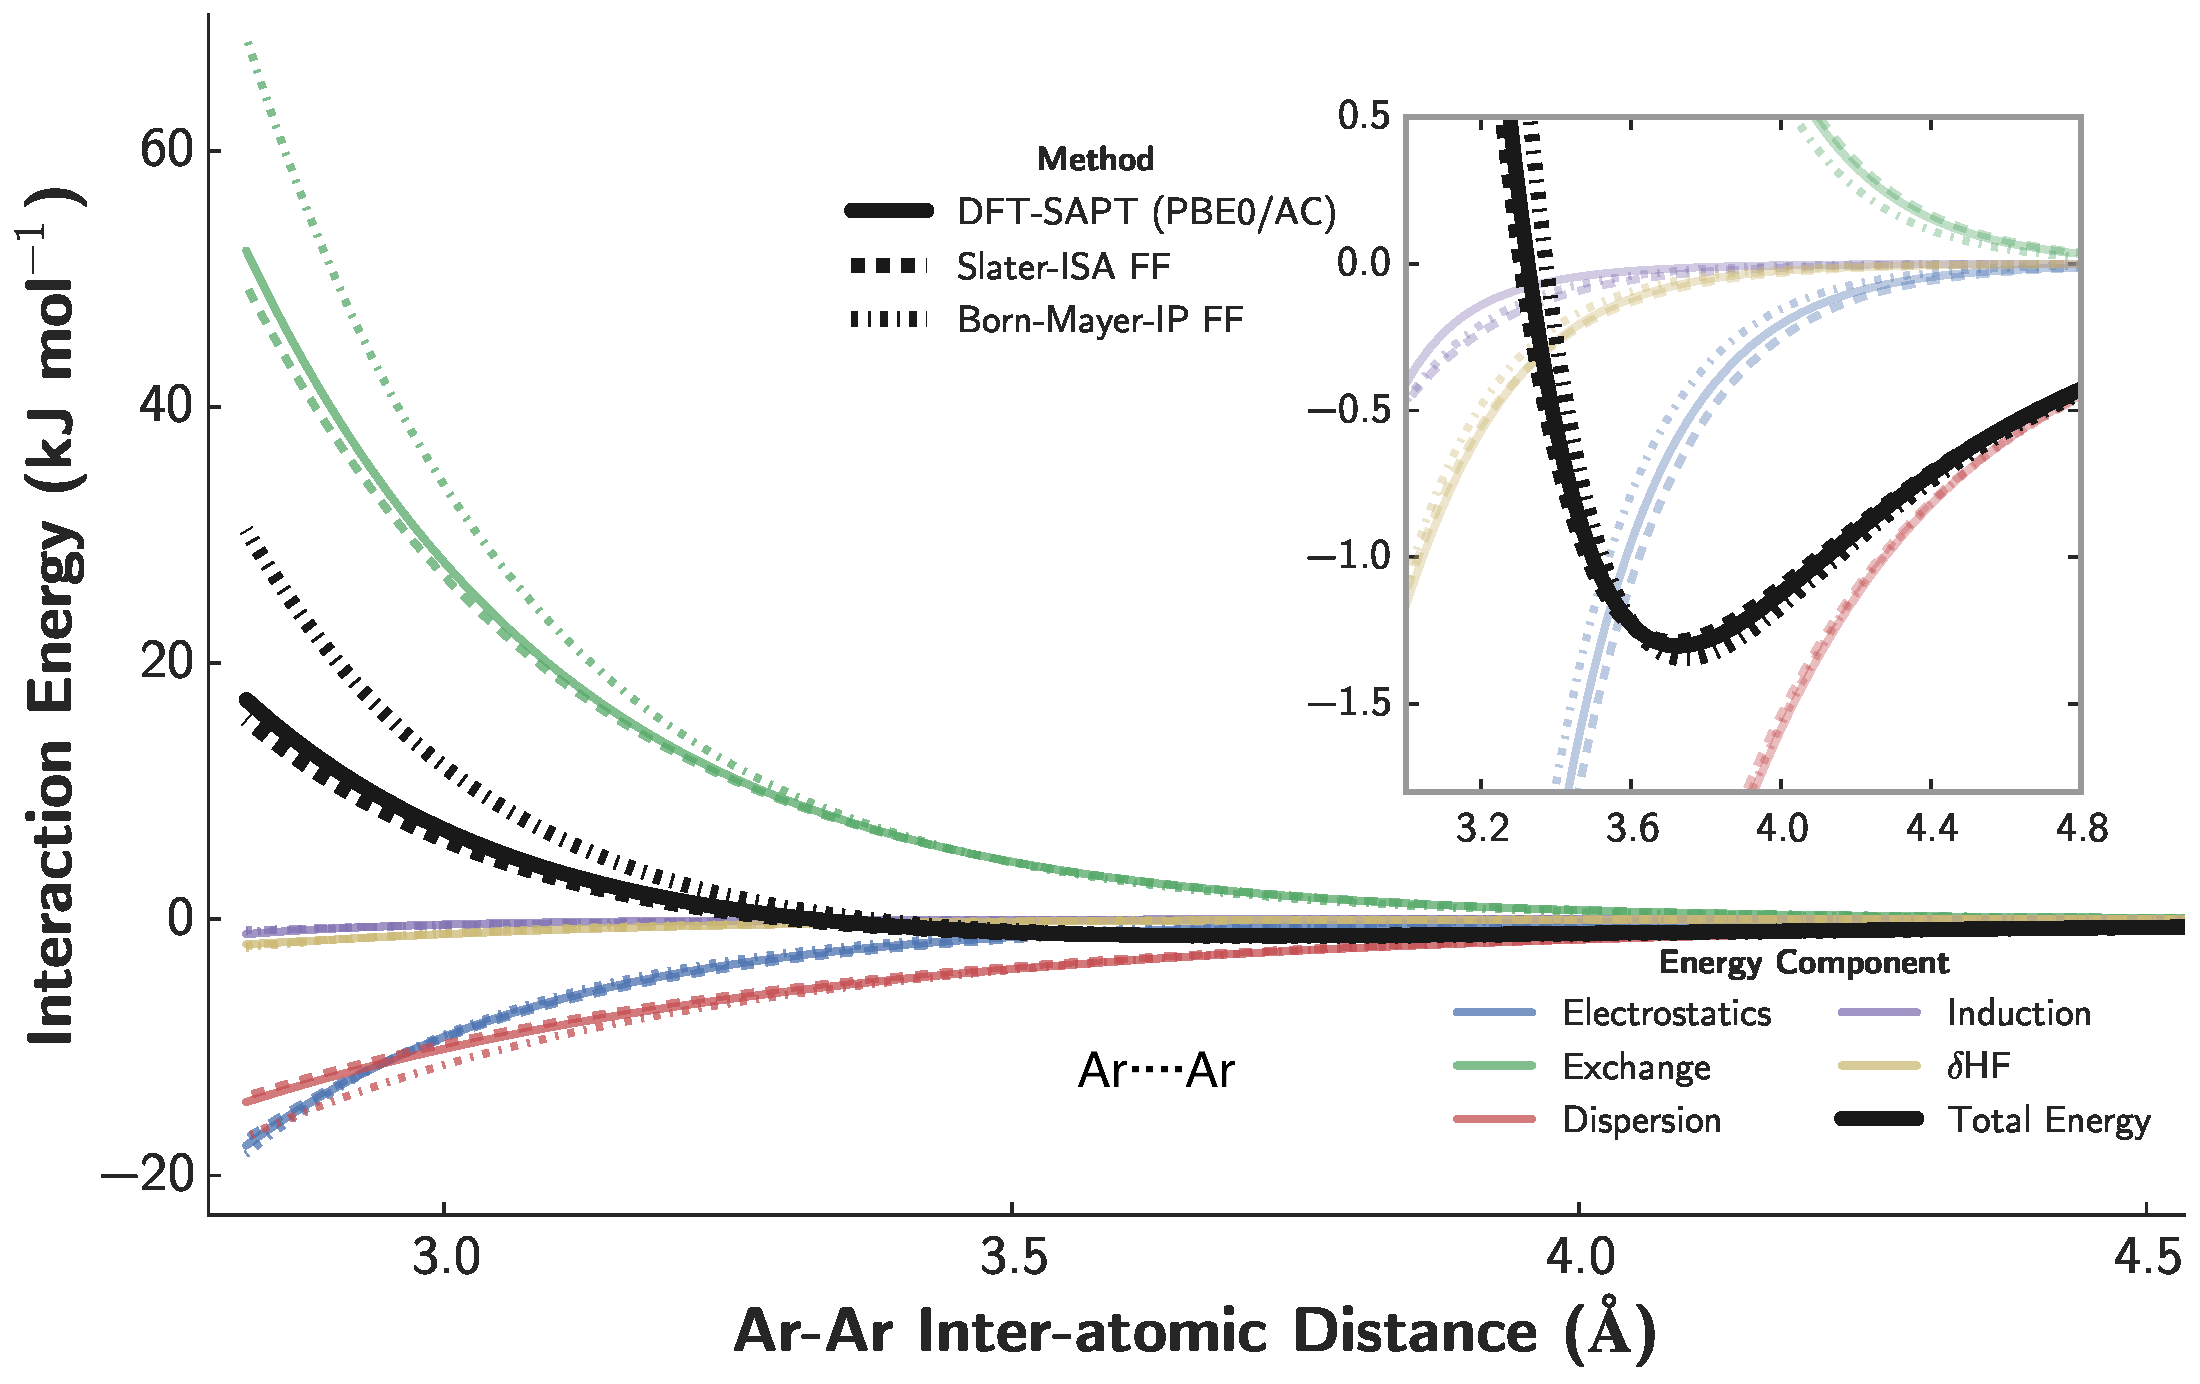
\includegraphics[width=0.9\textwidth]{isotropic/ar_ar_pes.pdf}
    \caption{
    Potential energy surface for the argon dimer. 
    Interaction energies for the \isaffold (dashed curves) and the \saptff (dash-dotted
    curves) are shown alongside benchmark \saptpbeo energies (solid curves). The
    energy decomposition for DFT-SAPT and for each force field is shown for reference.
    }
    \label{fig:isotropic-ar-pes}
    \end{figure}
    %%%%%%%%%%%% Ar-Ar PES %%%%%%%%%%%%%%%%%%

Results for \ljff are shown in the Supporting Information of
\citen{VanVleet2016}; consistent with expectations for the
Lennard-Jones model, the repulsive wall is overestimated by the
$1/r_{ij}^{12}$ short-range functional form, and the magnitude of the
attractive tail region is similarly overestimated by the effective $C_{ij,6}$
dispersion parameter. 
%
Note that this $C_{ij,6}$ coefficient has been fit to the total energy, and thus differs
from the asymptotically-correct $C_{ij,6}$ parameter used for both the \isaffold
and the \saptff. 
An alternative parameterization strategy would have been to use the asymptotically-correct $C_{ij,6}$
parameter in the \ljff, but this would have worsened predictions
along both the repulsive wall and the
minimum energy configurations.


\end{subsubsection}
\begin{subsubsection}{Ethane Dimer}


We next discuss the ethane dimer and show both a scatter plot
of the 1000 dimer interactions (\cref{fig:isotropic-ethane-scatter}) and a cut through the
potential energy surface near the minimum (\cref{fig:isotropic-ethane-pes}) as
indications of force field quality.

    %%%%%%%% Ethane-Ethane Scatter %%%%%%%%%%
    \begin{figure}
    %\includegraphics[width=0.9\textwidth]{ammonia_ff_quality.png}
    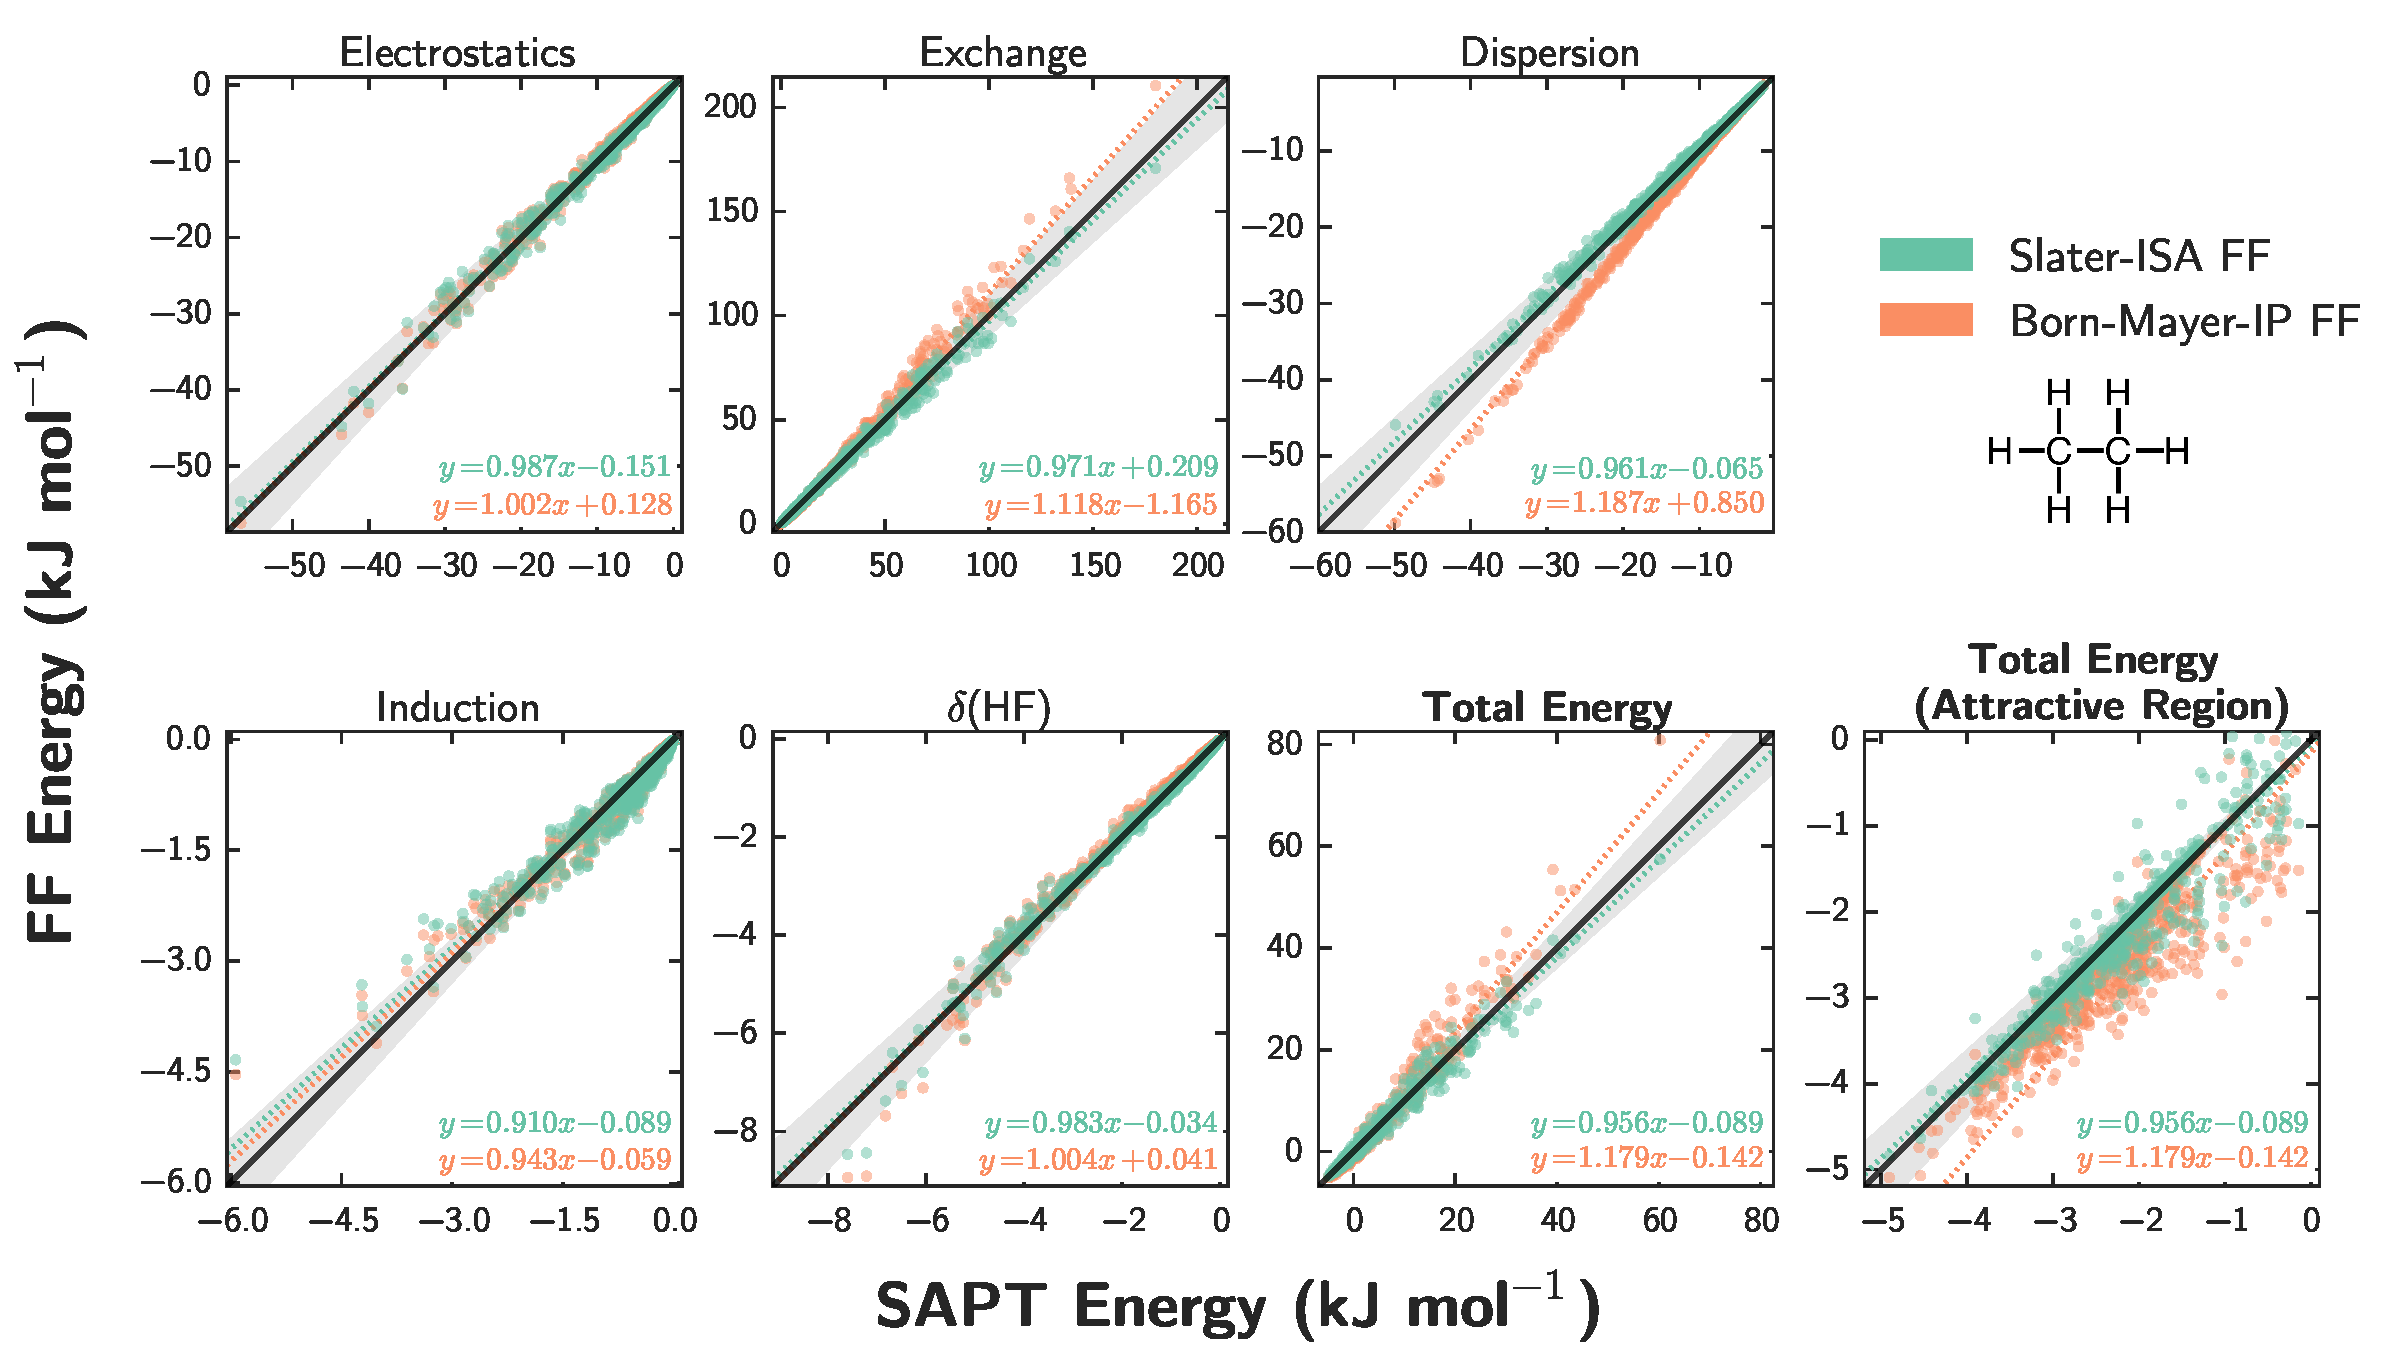
\includegraphics[width=0.9\textwidth]{isotropic/ethane_ethane_scatter.pdf}
    \caption{
    Force field fits for the ethane dimer using the Slater-ISA (green) and
    Born-Mayer-IP (orange) FFs.
    Fits for each energy component are displayed along with two views of the total interaction energy.
    The diagonal line (black) indicates perfect agreement between reference energies
    and each force field, while shaded grey areas represent points within $\pm
    10\%$ agreement of the benchmark. To guide the eye, a line of best fit (dotted
    line) has been computed for each force field and for each energy component.
     }
    \label{fig:isotropic-ethane-scatter}
    \end{figure}
    %%%%%%%% Ethane-Ethane Scatter %%%%%%%%%%

As with the argon dimer, for the ethane dimer the \isaffold produces more
accurate exchange and dispersion energies compared to the \saptff. Here, the
effects of the \isaffold for dispersion are even more pronounced, likely because
the conventional damping of the \saptff is systematically in error due to
differences in both the form of the damping function and exponents. As for the
total interaction energy, we again find that the \saptff exhibits large errors
for repulsive contributions, while the \isaffold naturally reproduces
interactions for both attractive and strongly repulsive configurations.  Even
in the attractive regime, the \saptff is systematically too attractive. These
systematic errors are the result of imperfect error cancellation
between the exchange and dispersion components of the fit, and are discussed in
more detail in Section \ref{sec:isotropic-results-robustness}. 

    %%%%%%%%%%% Ethane-Ethane PES %%%%%%%%%%%
    \begin{figure}
    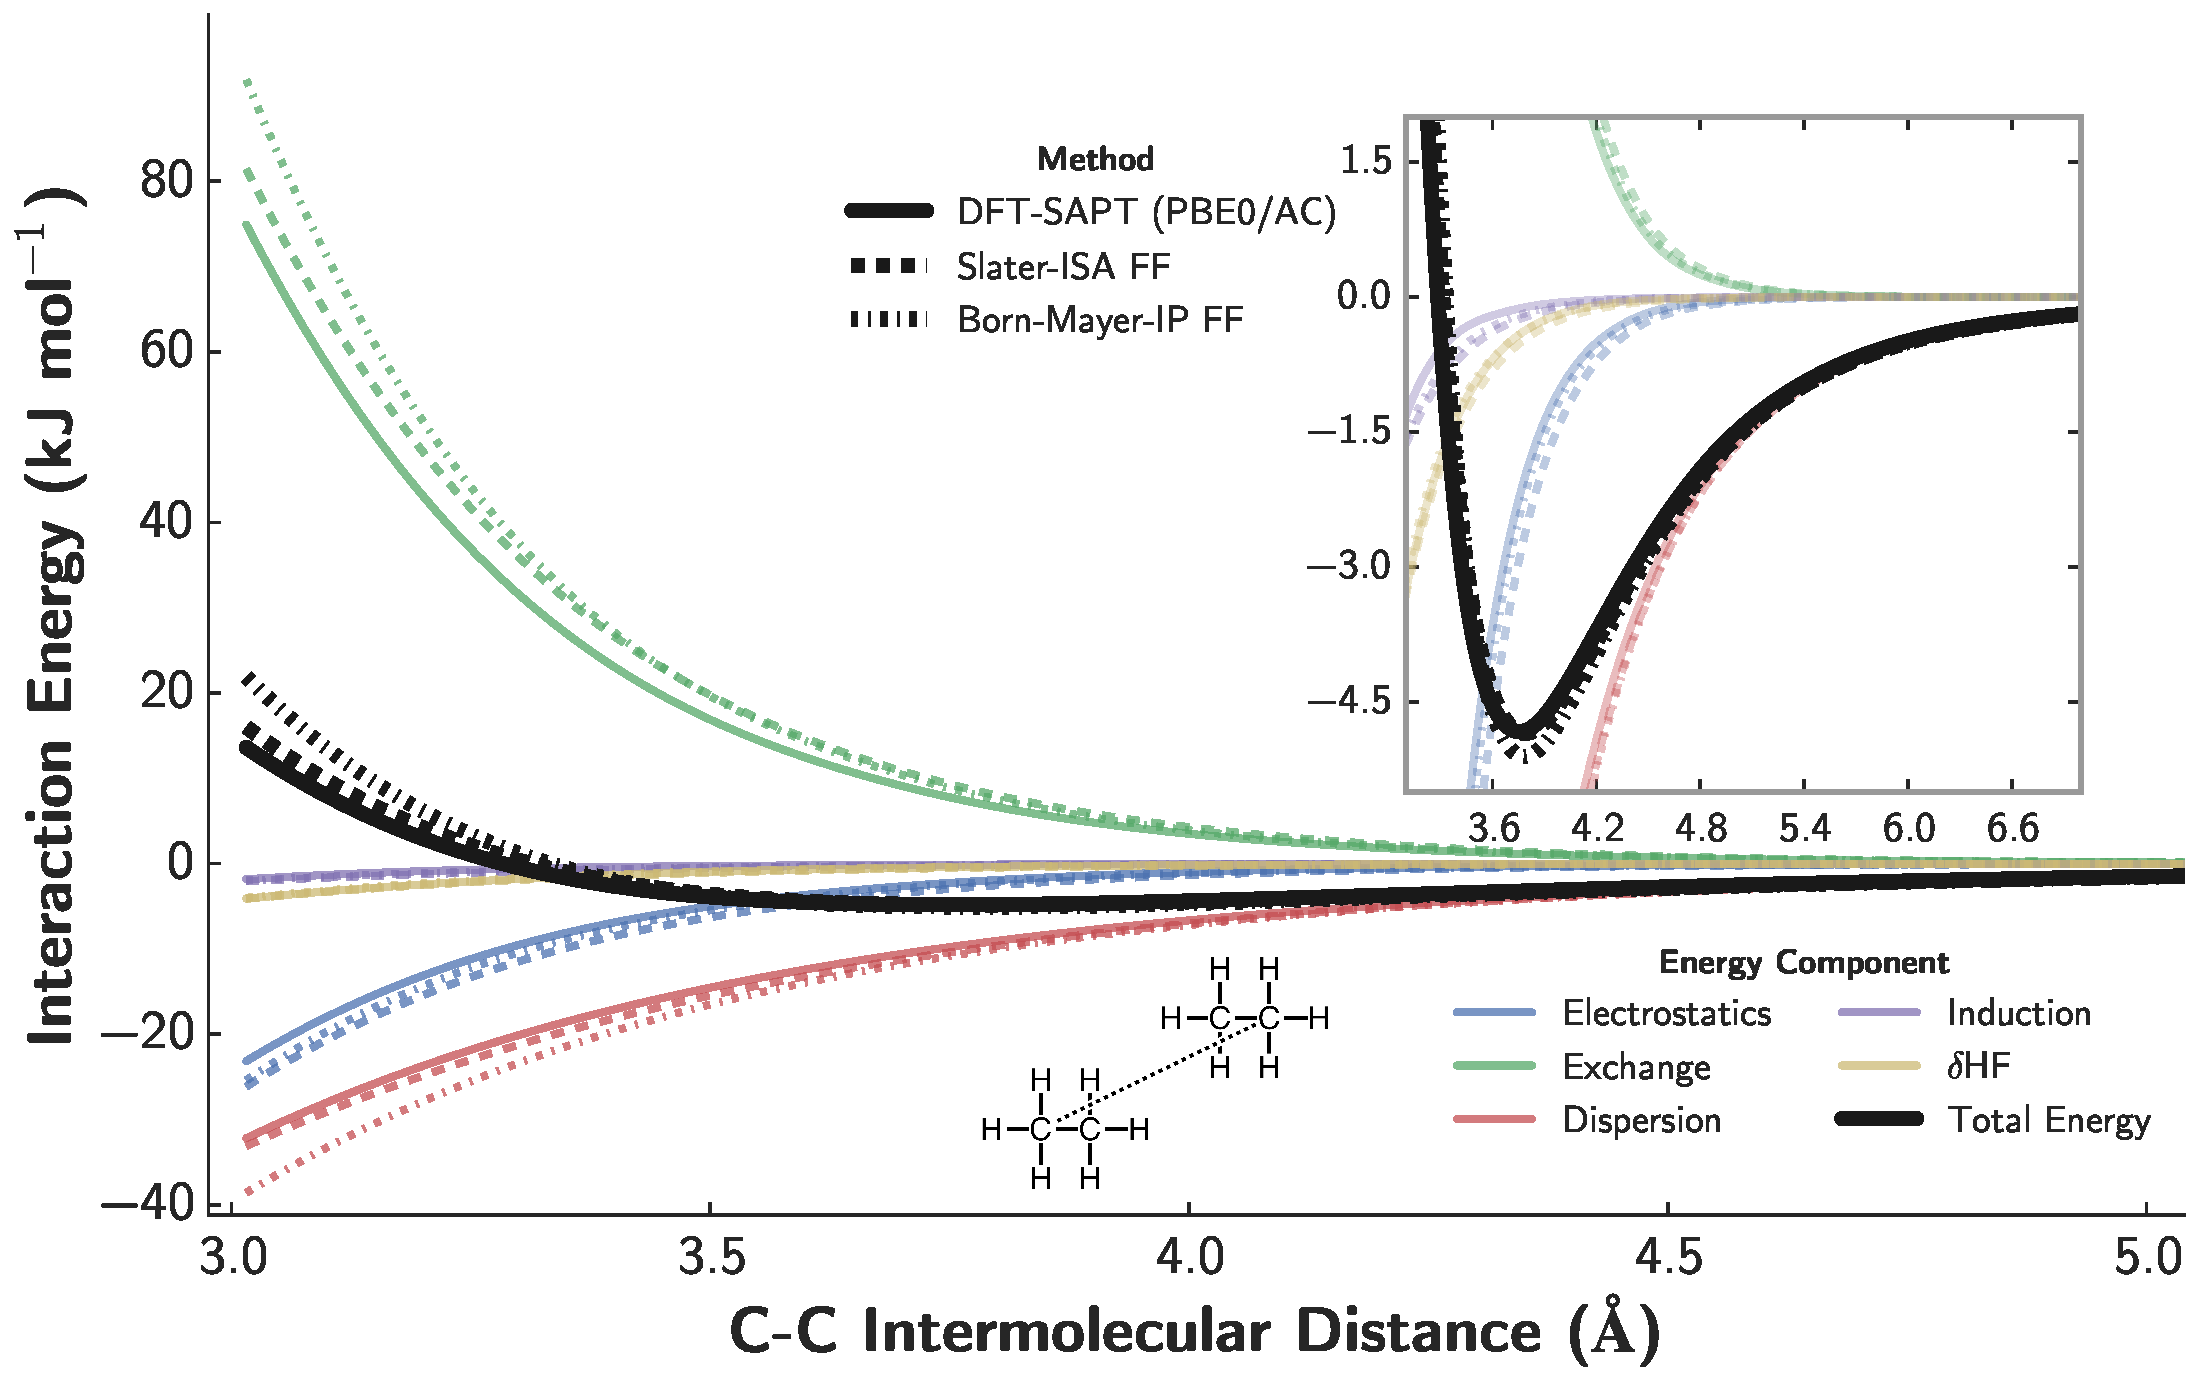
\includegraphics[width=0.9\textwidth]{isotropic/ethane_ethane_pes.pdf}
    \caption{
    A representative potential energy scan near a local minimum for the ethane dimer. 
    Interaction energies for the \isaffold (dashed curves) and the \saptff (dash-dotted
    curves) are shown alongside benchmark \saptpbeo energies (solid curves). The
    energy decomposition for DFT-SAPT and for each force field is shown for reference.
     The ethane dimer configuration in this scan corresponds to the most
    energetically attractive dimer included in the training set; other
    points along this scan are not included in the training set.
    }
    \label{fig:isotropic-ethane-pes}
    \end{figure}
    %%%%%%%%%%% Ethane-Ethane PES %%%%%%%%%%%

Examining a specific cut across the ethane-ethane PES
(\cref{fig:isotropic-ethane-pes}) visually confirms these results.  Both potentials do
an excellent job of reproducing the benchmark DFT-SAPT energies in the minimum
energy region, though the \saptff is slightly too attractive. (Other cuts of
the PES would show the Born-Mayer-IP predictions to be significantly more in error,
consistent with the scatter plots). Along the repulsive wall, however, the
\saptff predictions worsen in comparison to those from the \isaffold. Finally,
the PES shows an increased reliance on error cancellation between the
various energy components for the \saptff compared to the \isaffold.

As shown in the Supporting Information of \citen{VanVleet2016}, the Lennard-Jones force field models
are incapable of reproducing the entirety of the ethane PES; depending on the
weighting function, either the repulsive wall or the attractive well can be
reproduced, however no set of parameters can predict both regions
simultaneously.


\end{subsubsection}
\begin{subsubsection}{Acetone Dimer}

The acetone dimer provides a final interesting example involving a moderately sized
organic molecule.
From both the scatter plots (\cref{fig:isotropic-acetone-scatter}) and the PES cross section
(\cref{fig:isotropic-acetone-pes}), it is evident that both the Slater-ISA and
Born-Mayer-IP force fields do an
excellent job of reproducing DFT-SAPT energies for the low energy dimers.
Along the repulsive wall, however, the \saptff shows larger systematic
errors in each energy component, and seems to rely on error cancellation
to achieve good agreement in the total energy.
This reliance on error cancellation has two negative effects: 
Firstly, the additional scatter in the total energy of the \saptff
fit, especially prominent for attractive configurations, indicates that this
error cancellation is imperfect in certain cases. MSE
for the \isaffold ($-0.0115$ kJ mol$^{-1}$) are an order of magnitude lower than for
the \saptff ($0.182$ kJ mol$^{-1}$) in the attractive region of the potential.  Secondly,
as we shall later explore, reliance on error cancellation likely
contributes to the somewhat decreased transferability of the \saptff as
compared to the \isaffold. 

As shown in the Supporting Information of \citen{VanVleet2016}, the
\ljff predictions for acetone are reasonably good in both the tail and minimum
energy regions of the potential, however the \ljff grossly overpredicts the
\saptpbeo energies along the repulsive wall.

    %%%%%%% Acetone-Acetone Scatter %%%%%%%%%
    \begin{figure}
    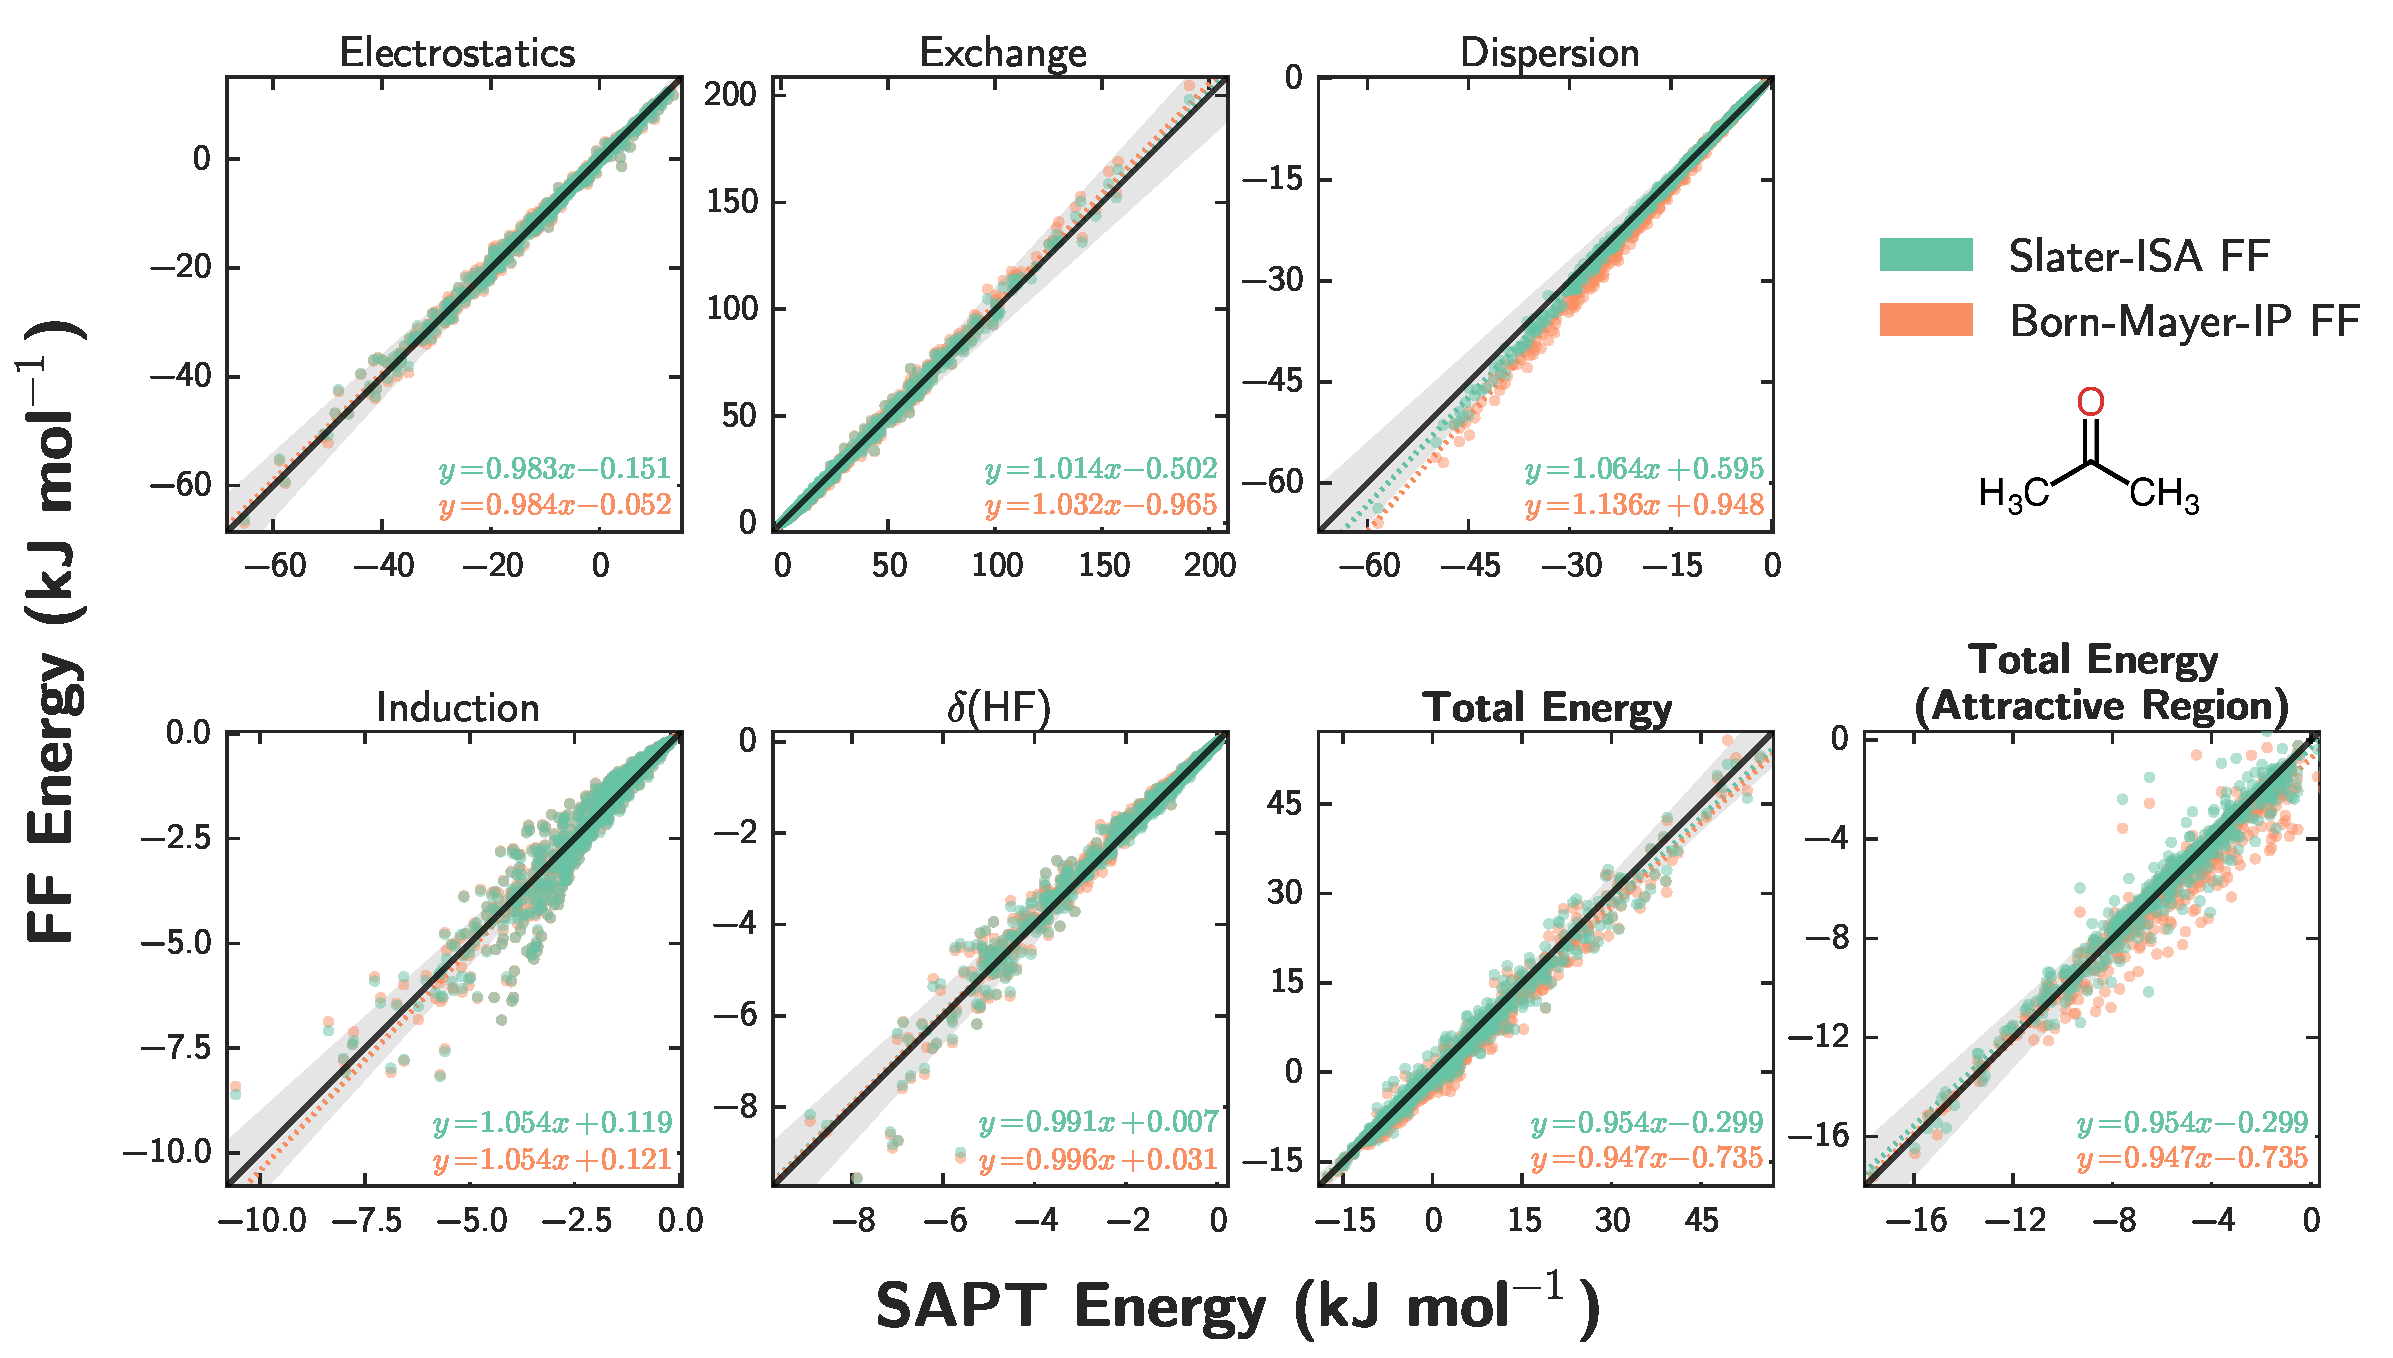
\includegraphics[width=0.9\textwidth]{isotropic/acetone_acetone_scatter.pdf}
    \caption{
    Force field fits for the acetone dimer using the Slater-ISA (green) and
    Born-Mayer-IP (orange) FFs, as in \cref{fig:isotropic-ethane-scatter}.
    %% Fits for each energy component are displayed along with two views of the total interaction energy.
    %% The diagonal line (black) indicates perfect agreement between reference energies
    %% and each force field, while shaded grey areas represent points within $\pm
    %% 10\%$ agreement of the benchmark. To guide the eye, a line of best fit (dotted
    %% line) has been computed for each force field and for each energy component.
            }
    \label{fig:isotropic-acetone-scatter}
    \end{figure}
    %%%%%%% Acetone-Acetone Scatter %%%%%%%%%


    %%%%%%%%%%% Acetone-Acetone PES %%%%%%%%%
    \begin{figure}
    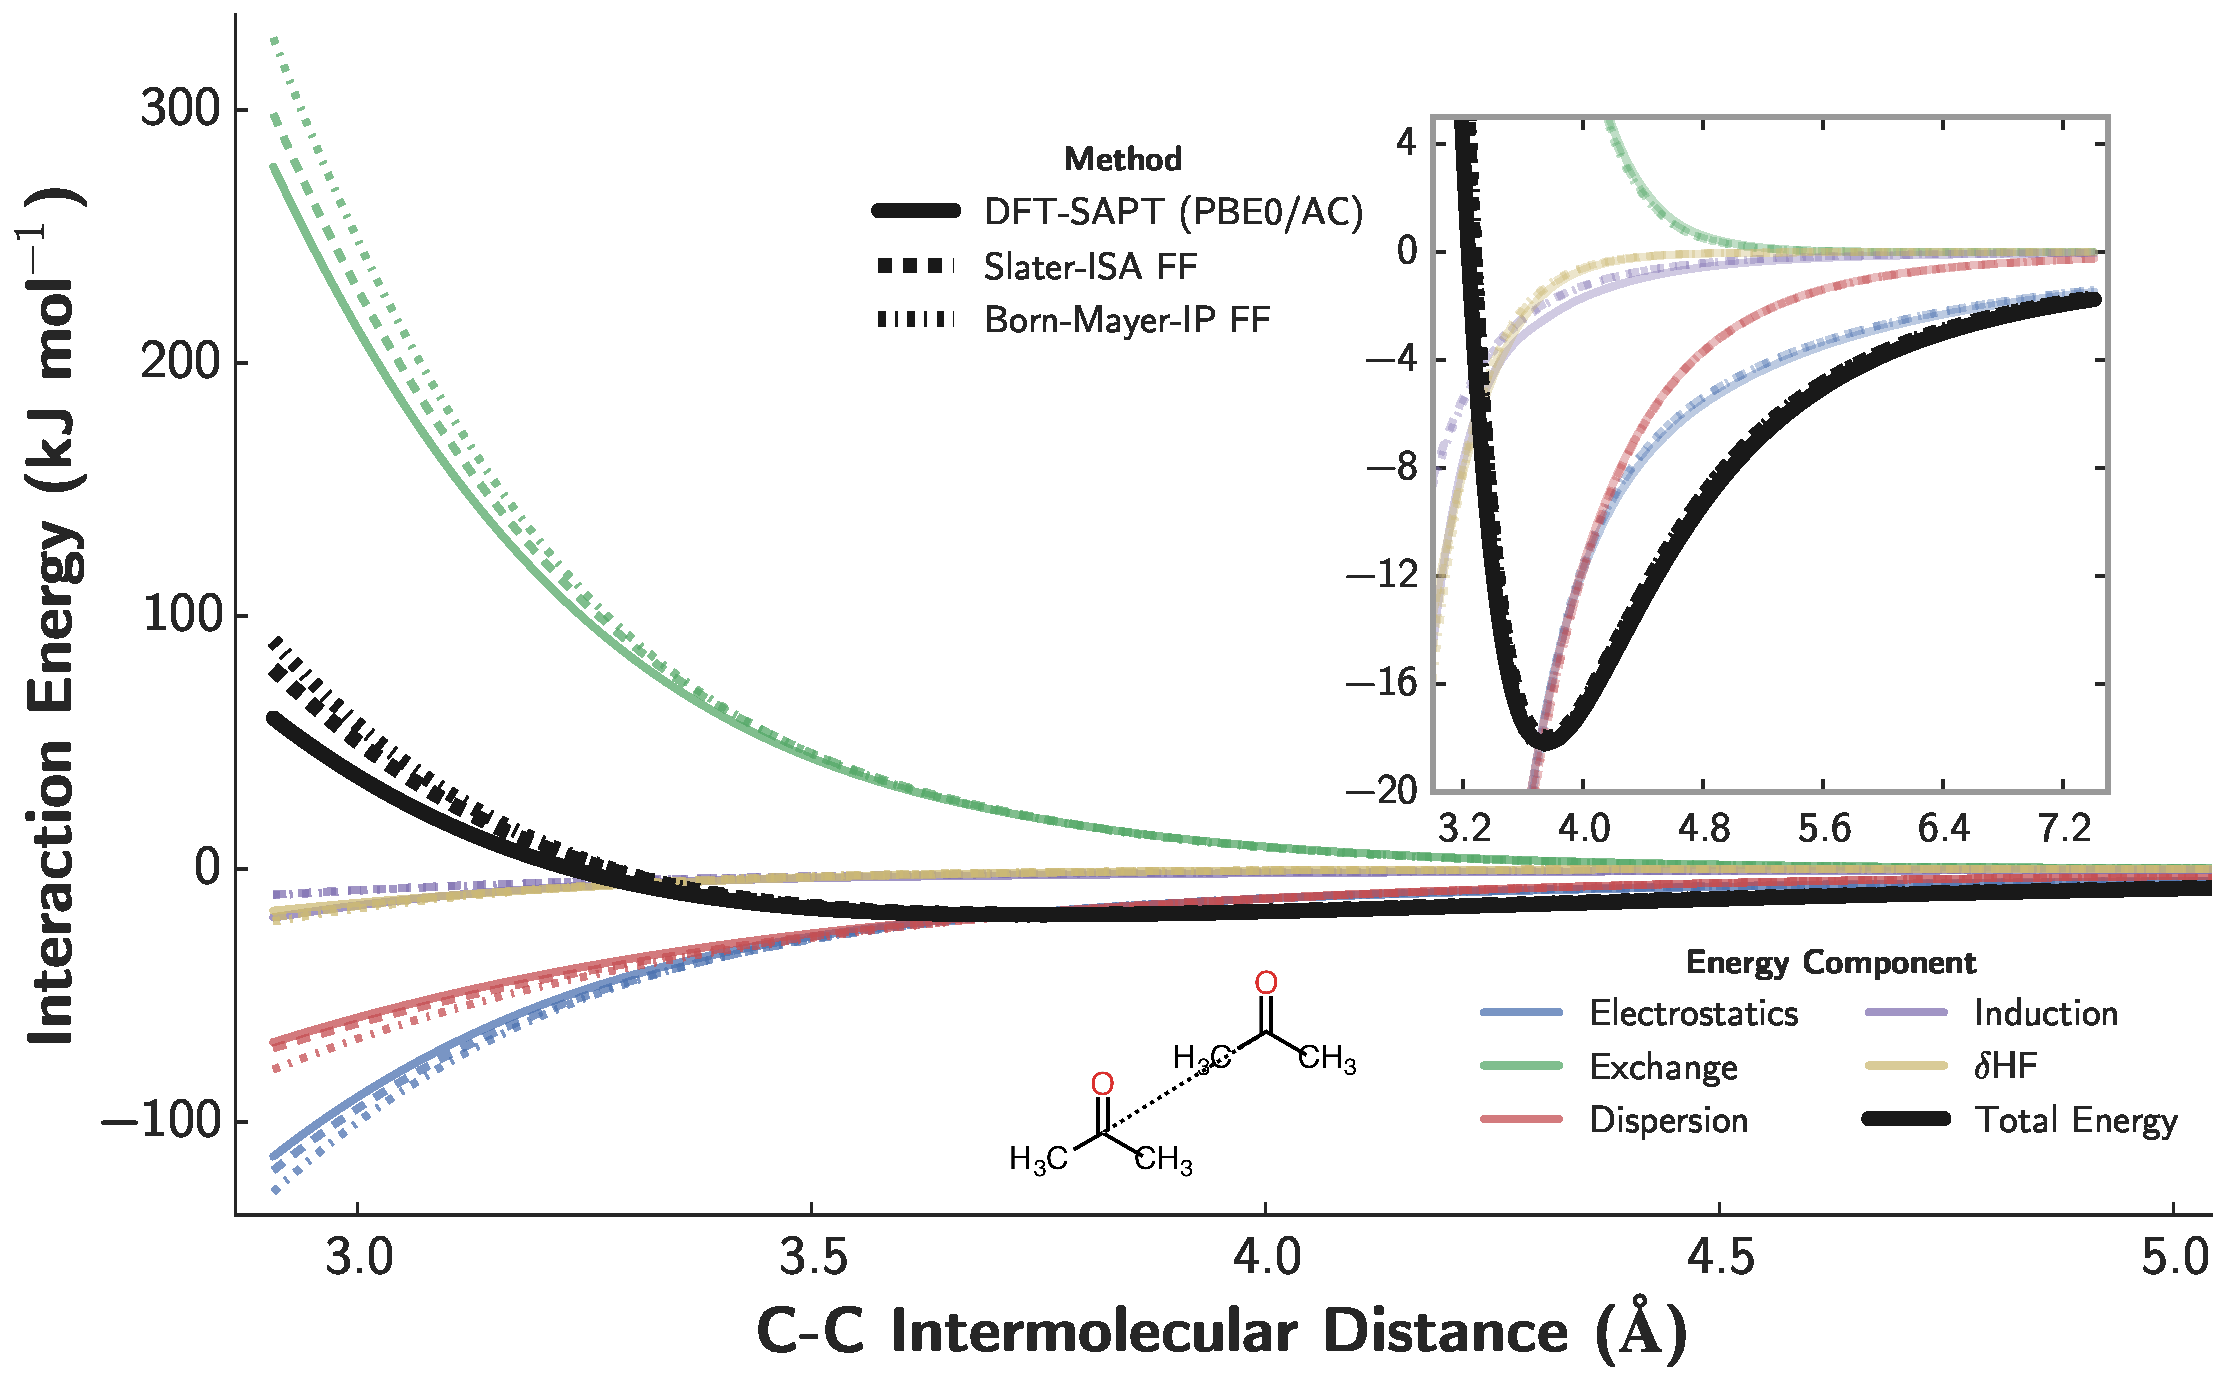
\includegraphics[width=0.9\textwidth]{isotropic/acetone_acetone_pes.pdf}
    \caption{
      A representative potential energy scan near a local minimum for the
      acetone dimer.  Interaction energies for the \isaffold (dashed curves) and
      the \saptff
      (dash-dotted curves) are shown alongside benchmark \saptpbeo energies (solid
      curves). The energy decomposition for DFT-SAPT and for each force field is
      shown for reference.  The intermolecular distance is taken to be the
      internuclear distance between the two carbonyl carbons on each acetone
      monomer.  The configuration in this scan corresponds to the
      most attractive dimer configuration included in the training set for the acetone dimer;
      other points along this scan have not explicitly been included in the training
      set.
      }
    \label{fig:isotropic-acetone-pes}
    \end{figure}
    %%%%%%%%%%% Acetone-Acetone PES %%%%%%%%%


\end{subsubsection}
\end{subsection}
\begin{subsection}{Accuracy: Comparison with experiment}
\label{sec:isotropic-accuracy_experiment}


    %%%%%%%%%%%% Ar-Ar Virial %%%%%%%%%%%%%%%
    \begin{figure}
    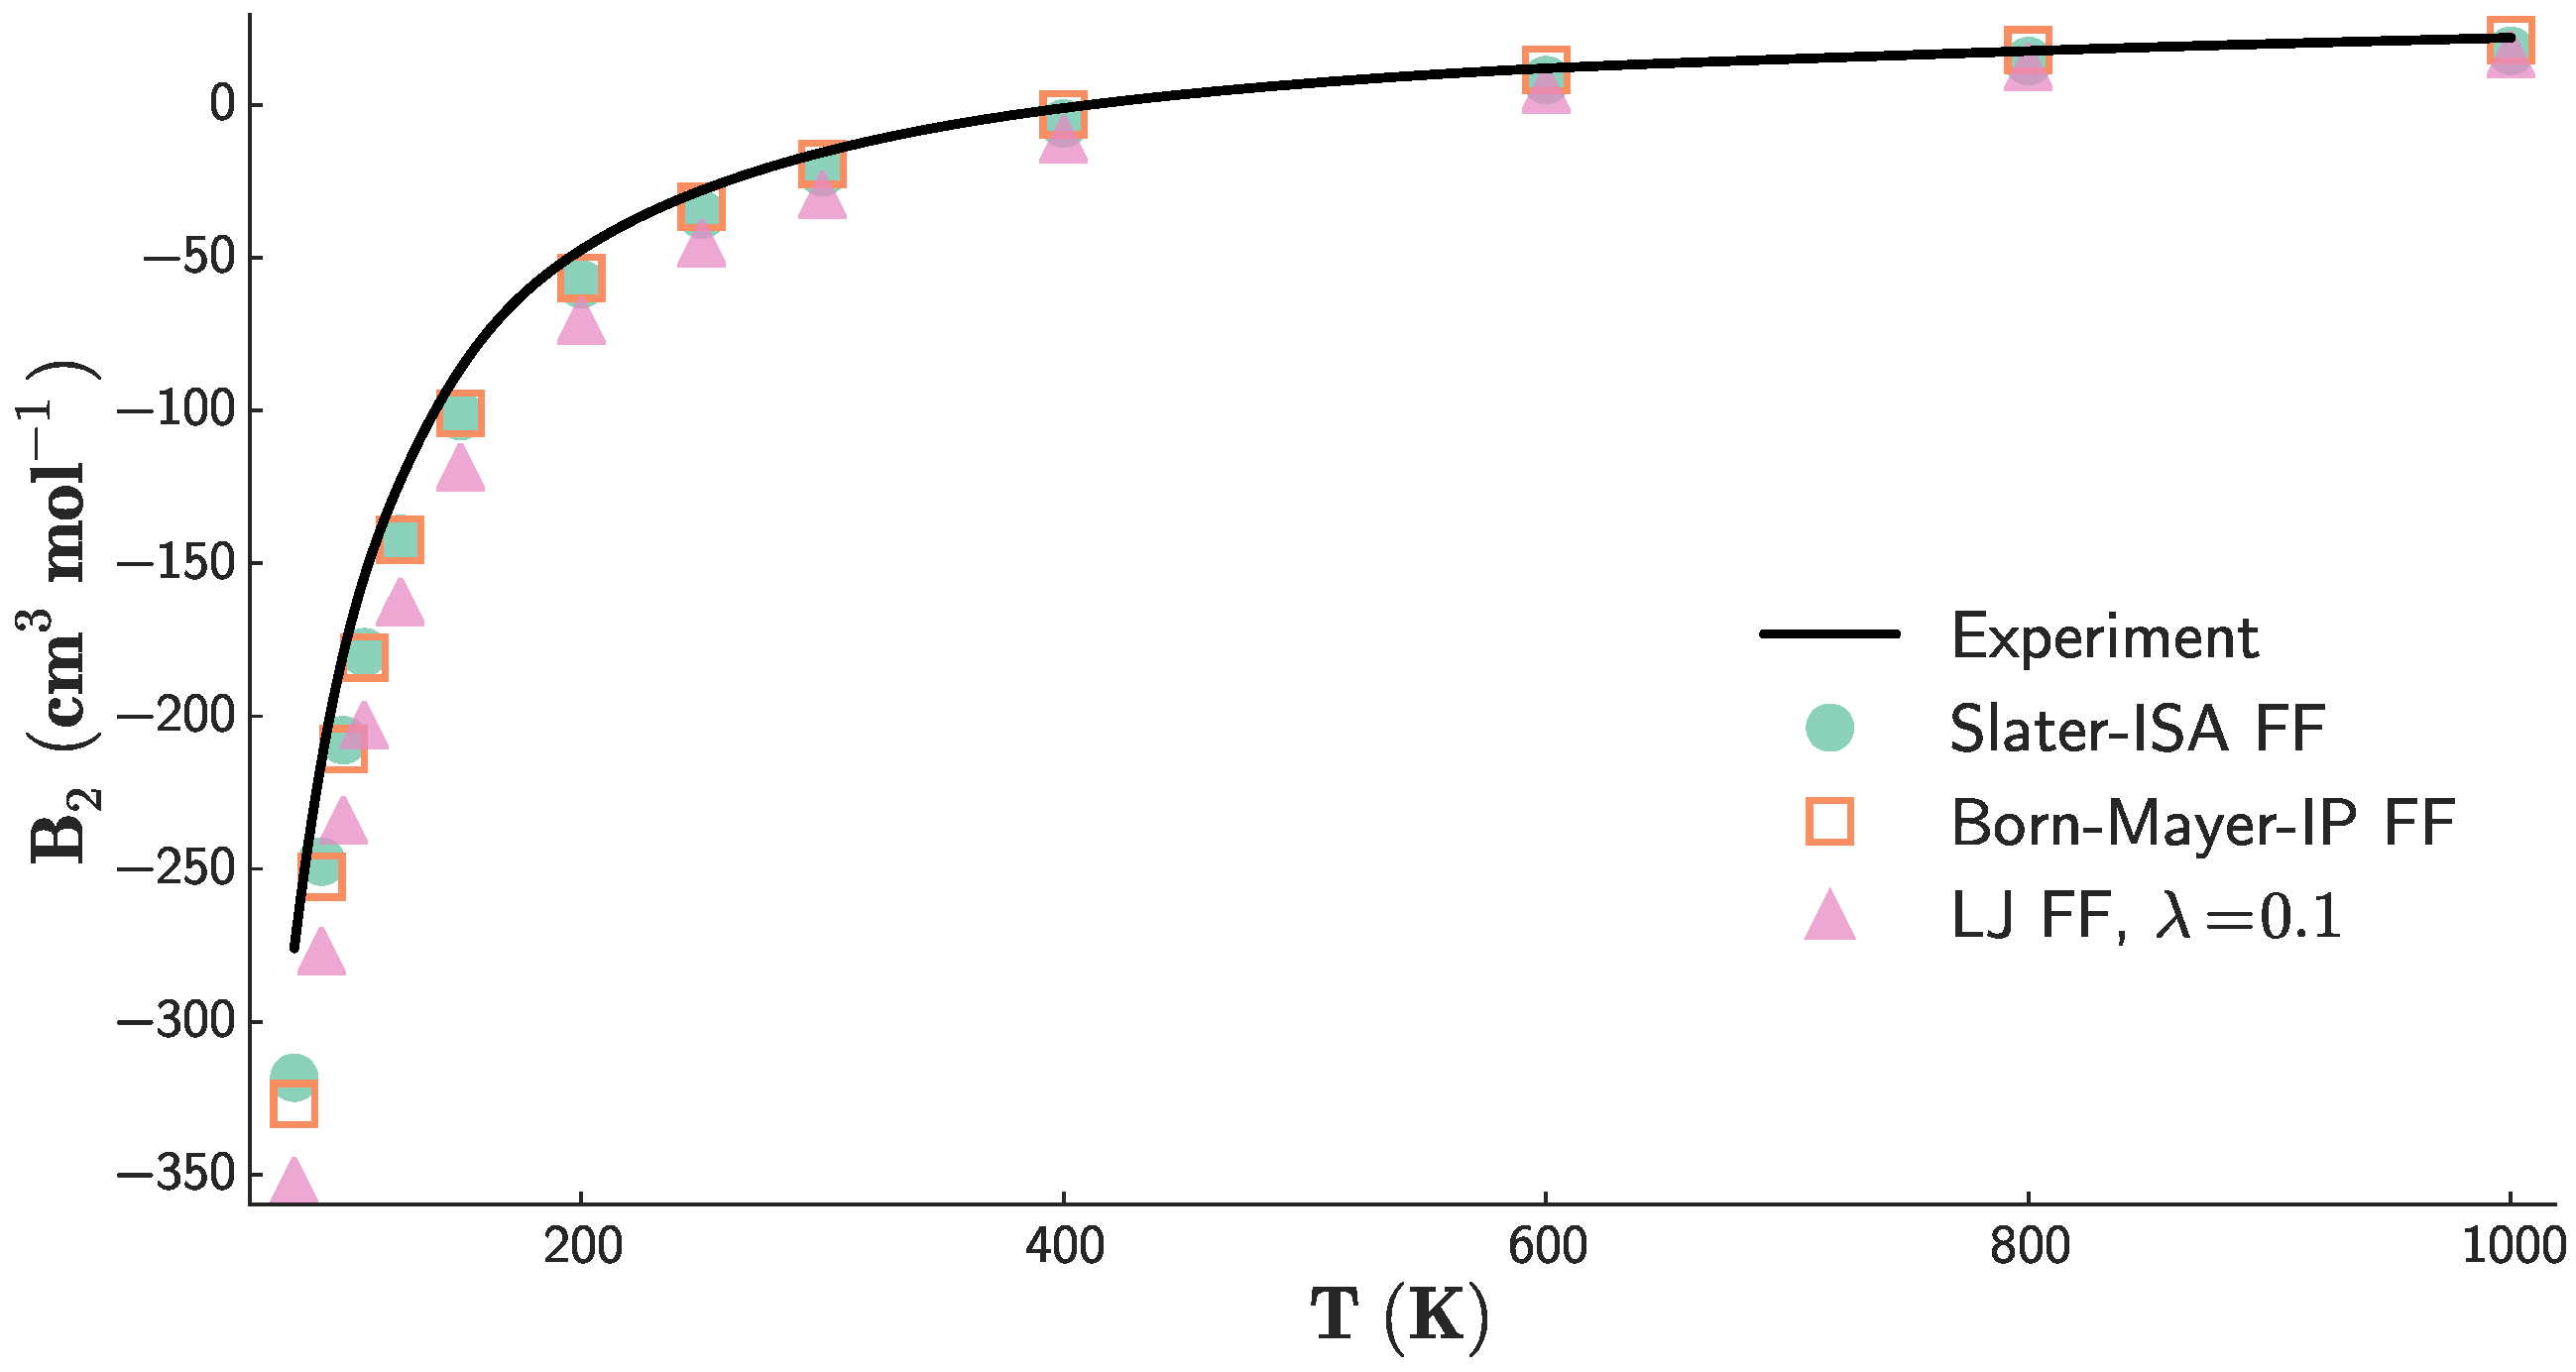
\includegraphics[width=0.9\textwidth]{isotropic/ar_2nd_virial_wi_lj.pdf}
   \caption{
    Second virial coefficients for argon. The Slater-ISA and the Born-Mayer-IP
    FFs are shown as green
    circles and orange squares, respectively; the black line corresponds to
    experiments from \citen{Dymond1980}.
           }
    \label{fig:isotropic-ar-virial}
    \end{figure}
    %%%%%%%%%%%% Ar-Ar Virial %%%%%%%%%%%%%%%

We have benchmarked the above force fields against experimental 
second virial coefficients and, in the case of ethane, enthalpies of
vaporization and liquid densities.
The classical 2\super{nd} virial coefficients were calculated for both argon and
ethane using rigid monomer geometries, following the procedure described in
\citen{McDaniel2013}. 
Enthalpies of
vaporization and liquid densities were calculated using the OpenMM molecular
simulation package
\cite{Eastman2013}
as described in \cref{sec:isotropic-methods}.
Higher-order multipole moments
--- which were negligible for these molecules --- were neglected, and so
only rank $0$ terms were used in these calculations. 
Results are shown in Figures \ref{fig:isotropic-ar-virial} and \ref{fig:isotropic-ethane-virial}
as well as \cref{tab:isotropic-deltah}.


For argon, since both \isaffold and \saptff accurately reproduce the energetics 
of low-energy configurations, it
is unsurprising that both force fields yield accurate virial
coefficients over a wide range of temperatures.  Errors in computed $B_2$
coefficients (for both potentials) are likely attributable to small errors in
the \saptpbeo potential itself,
\cite{Podeszwa2005a}
and, to a much lesser extent, the neglect of nuclear
quantum effects at lower temperatures.
\cite{Vogel2010}
Despite the good (in an RMSE sense) fit quality of the \ljff ($\lambda=0.1$),
this force field overpredicts the magnitude of the 2\super{nd} virial for argon, likely as a
result of the effective dispersion coefficient, which overestimates the
attraction in the tail
region of the PES (see Supporting Information of \citen{VanVleet2016}). Although it is certainly
possible to parameterize a Lennard-Jones model \emph{empirically} for argon,
such a force field would rely on a subtle cancellation of errors between the
minimum energy- and tail-regions of the PES. As the proper balance is
impossible to predict a priori, this result highlights one of the difficulties
of using the less physical LJ model in the development of ab-initio force
fields.

%
    %%%%%%%% Ethane-Ethane Virial %%%%%%%%%%%
    \begin{figure}
    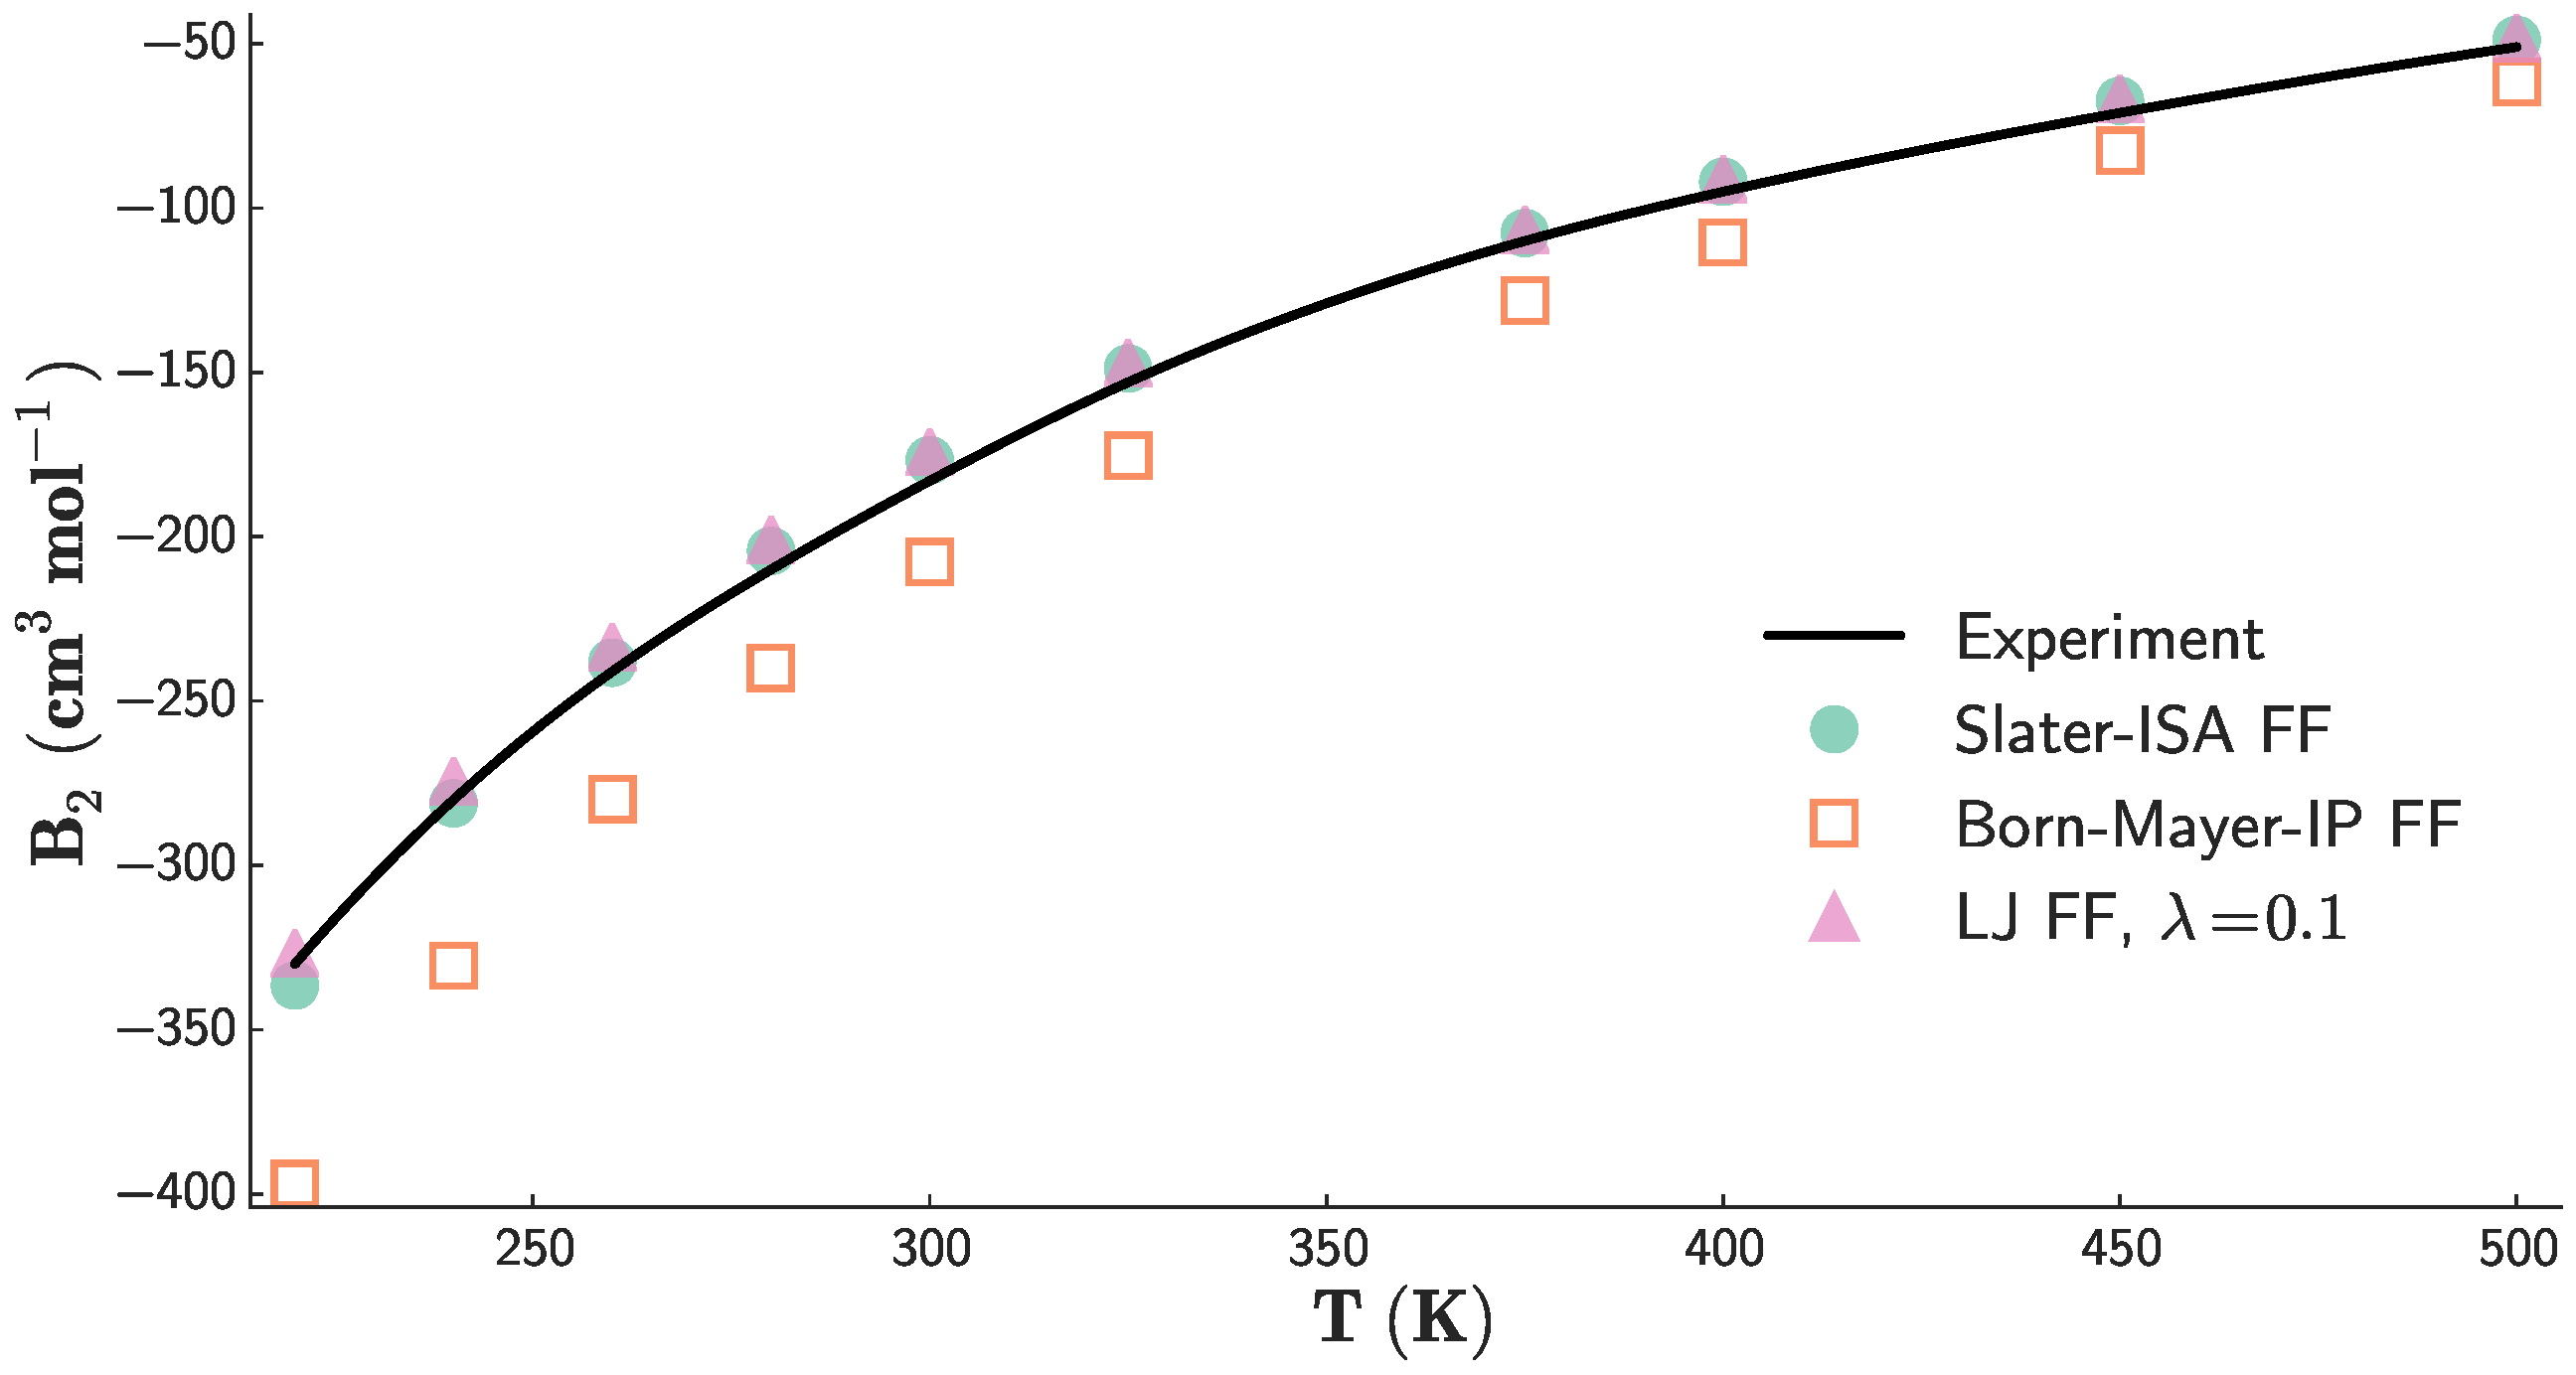
\includegraphics[width=0.9\textwidth]{isotropic/ethane_2nd_virial_wi_lj.pdf}
   \caption{
    Second virial coefficients for ethane. 
    The Slater-ISA and Born-Mayer-IP FFs are shown as green
    circles and orange squares, respectively; the black line corresponds to
    experiments from \citen{Dymond1980}.
    }
    \label{fig:isotropic-ethane-virial}
    \end{figure}
    %%%%%%%% Ethane-Ethane Virial %%%%%%%%%%%
%

In the case of ethane, the \isaffold is in excellent agreement with experiment,
whereas the \saptff underpredicts $B_2$ by as much as 20\%. These results are
indicative, not only of the more accurate functional form and parameterization
of \isaffold, but also of the high accuracy of the underlying \saptpbeo benchmark
energies. In this case, \ljff also correctly predicts the virial.  Using
weighting functions for each model that are optimal for the 91 dimer test set
as a whole ($\lambda = 2.0$ for the \isaffold and the \saptff,
$\lambda = 0.1$ for the \ljff), all force fields produce similar results for
$\Delta H_{\text{vap}}$ and $\rho$ (\cref{tab:isotropic-deltah}). These values are
slightly overestimated by all force fields (especially in the case of the
\saptff), which is to be expected given our neglect of many-body effects.
\citeauthor{McDaniel2014} have calculated the 3-body correction for the
\saptff; using this value as a global 3-body correction for all force fields,
we see that both the Slater-ISA and the Lennard-Jones force fields compare
very favorably to experiment, with the \isaffold perhaps slightly more accurate. 
%TO-DO: Update this once I have saptpbeo-ff results.

\end{subsection}

\begin{subsection}{Transferability}
\label{ss:transferability}

The transferability of interaction potentials is a crucial aspect of practical
molecular simulations. Here we examine `parameter transferability', by which
we mean the extent to which parameters from two homo-monomeric systems can
combined to predict the intermolecular interactions of the resulting mixed
hetero-monomeric system. 
As a measure of parameter transferability, we compared characteristic RMSE
and \mse relative to
the benchmark data for two different parameterization schemes.  For the
`Dimer-Specific Fits', \A parameters were obtained for each of the 91 dimer
pairs individually; these results are identical to those discussed in the
previous two subsections. In contrast, for the `Transferable Fits', the \A
parameters were fit to the 13 homonomeric dimer pairs and were re-used
(without any further optimization) to calculate energies for the 78 mixed
systems using the combination rules listed in \cref{sec:isotropic-FF-forms}.
Results for each parameterization scheme are shown in \cref{tab:isotropic-rmse}. 
From the RMSE and \mse from the competing schemes, 
we see excellent parameter transferability for all force fields studied. 
For the \isaffold, characteristic RMSE and \mse for each component increase by a very small
fraction upon constraining the fit; due to small error cancellation, errors in the
total energy actually \emph{decrease} somewhat with these constraints. 
(This is possible since the total energy is not directly fit.)
The \saptff also displays a significant degree of transferability, though
errors in the total energy increase slightly upon constraining the fit.
As in prior work, the observed parameter transferability for both force fields can be
attributed to our use of a term-by-term parameterization scheme
(\cref{sec:isotropic-FF-forms}),
which serves to minimize error cancellation between energy components and generate a
more physically-meaningful (and thus transferable) set of parameters.
\cite{McDaniel2013,McDaniel2012a}
Finally, note that for four of the five interaction energy components the relative
change in RMSE on constraining the fit is smaller for the \isaffold than
the \saptff. The \dhf term is the exception, but even here the relative 
change in errors from the two methods are comparable. This suggests that the
\isaffold may be the more transferable of the force fields studied.
Nevertheless, the Lennard-Jones model is surprisingly transferable,
likely in part due to the same accurate and transferable `long-range'
electrostatics and polarization as the \isaffold. The non-polarizable, point-charge
Lennard-Jones model (results for which are shown in the Supporting
Information of \citen{VanVleet2016}) displays the least transferability (in both an RMSE and \mse
sense) of all force fields studied.

Although we do not examine it here, we expect that the previously demonstrated success\cite{McDaniel2013, McDaniel2012,
McDaniel2012a, McDaniel2014} of the \saptff with respect to `environment transferability'
--- the extent to which a single set of parameters can model a variety of phases and
molecular environments --- and `atom type transferability' --- the extent to which
atoms in chemically similar environments can accurately be grouped together
into `types' and treated using one parameter set --- 
would also apply to, or even be improved by, \isaffold. These issues are under
investigation in our groups.

\end{subsection}
\begin{subsection}{Robustness}
\label{sec:isotropic-results-robustness}


One of the practical challenges of ab initio force field development is the
robustness of the resulting force field quality with respect to the choice of an
appropriate training set and/or weighting function.  To this end, the default
weighting function (\cref{eq:isotropic-weighting-function}, $\lambda = 2.0$) was varied
to produce unconstrained fits that were skewed either towards attractive
($\lambda = 0.5$) or repulsive ($\lambda = 5.0$) configurations, and pairwise
differences in force field total energies were computed between each weighting
scheme. Characteristic root-mean-square pairwise differences (RMSD) between
each weighting function are shown in
\cref{tab:isotropic-rmsd-weightings}; as before, `attractive RMSD' were
calculated by excluding repulsive points from consideration. Note that, on
average, the default $\lambda = 2.0$ weighting scheme is optimal (in an RMSE
sense) for both the Slater-ISA and Born-Mayer-IP FFs.

Overall, both the \saptff and the \ljff display significant weighting function
sensitivity. This sensitivity is not surprising; as both force fields are
unable to reproduce the entirety of the potential energy surface, changing the
weighting scheme (or equivalently, the balance of configurations in the
training set) alters the parameters in the \saptff or the \ljff models quite 
substantially. Even excluding repulsive configurations, RMSD
of $\sim0.5$ kJ mol$^{-1}$ are typical for the \saptff. RMSD are
somewhat smaller for the \ljff ($\sim0.3$ kJ mol$^{-1}$), however
qualitatively we see that differences in computed force field energies are systematic: smaller weighting
functions capture the minimum energy region of the potential while
overestimating the magnitudes of both the repulsive and tail regions of the
potential, whereas larger weighting functions tend to underestimate the
minimum energy region in order to correctly reproduce the repulsive wall.
Consequently, the Lennard-Jones model shows weighting-function sensitivity in
a manner that is not entirely captured by the RMSD, but is instead
reflected in the greater sensitivity of the \ljff (as compared to the \saptff)
in the prediction of experimental properties (\emph{vide infra}).
 
Note that for practical force field development (as opposed to minimization of
overall RMSE), the default weighting scheme for the \saptff
and the \ljff is suboptimal for many dimers in the test set.  Because both the
\saptff and the \ljff must inherently compromise between accuracy near the
minimum and along the repulsive wall, the weighting function requires
system-specific fine-tuning in order to achieve proper balance. This
empiricism creates significant challenges in the development of ab initio force
fields.

%%%%%%%%%%%%%%%%%%%%% Average RMSD Table %%%%%%%%%%%%%%%%%%%%%%%%%%%%%%%%%%%
\begin{table}[t]
\footnotesize
\centering
\renewcommand\arraystretch{1.1}
\begin{tabular}{@{}rcccccc@{}}
\hline
\toprule
\multirow{2}{*}{Characteristic RMSD} & \phantom{ab} &
  {$\lambda = 0.5$ vs 2.0} & \phantom{ab} &
  {$\lambda = 0.5$ vs 5.0} & \phantom{ab} &
  {$\lambda = 2.0$ vs 5.0} \\
  & \phantom{ab} &
  (kJ mol$^{-1}$) & \phantom{ab} &
  (kJ mol$^{-1}$) & \phantom{ab} &
  (kJ mol$^{-1}$) \\
\midrule
\isaffold    & & 0.742 (0.207) & & 0.990 (0.273) & & 0.306 (0.086) \\
\saptff   & & 1.866 (0.409) & & 2.632 (0.550) & & 0.797 (0.153) \\
\ljff  & & 1.301 (0.216) & & 1.605 (0.309) & & 0.324 (0.099) \\
%\midrule
%\addlinespace                                                                                                           
\bmsisaff & & 0.611 (0.178) & & 0.810 (0.236) & & 0.293 (0.081) \\ 

\bottomrule
\hline
\end{tabular}
\caption{
    Characteristic RMS pairwise differences (RMSD) in force field total energies 
    for different weighting functions with $\lambda$ values as defined in
    \cref{eq:isotropic-weighting-function}; values shown are the (arithmetic mean,
    rather than geometric)
    RMSD across the 91 dimer test set.
    Characteristic `Attractive' RMSD (as defined
    in \cref{tab:isotropic-rmse}) are shown in parentheses to the right of each overall RMSD.
	}
\label{tab:isotropic-rmsd-weightings}
\end{table}
\normalsize
%%%%%%%%%%%%%%%%%%%%% Average RMSD Table %%%%%%%%%%%%%%%%%%%%%%%%%%%%%%%%%%%

By contrast, we find the \isaffold to be robust with respect to the choice of
weighting function due to its more balanced treatment of repulsive and
attractive regions of the potential energy surface.
Average RMSD for the \isaffold are between two to three \emph{times} smaller compared
to the \saptff, and the \isaffold is relatively insensitive to the choice of
weighting function. 
These conclusions hold for both attractive and overall RMSD.
As a result, the Slater-ISA model largely eliminates the need for empirical
fine-tuning of the weighting function, which in turn greatly simplifies the
parameterization process and allows for a more robust prediction of chemical
and physical properties. 

For the ethane dimer, \cref{fig:isotropic-ethane-weighting} shows overall
force field energies for both the Slater-ISA and Born-Mayer-IP FFs for three
weighting functions. Results for the Lennard-Jones models are shown in the SI,
and are qualitatively similar to the \saptff results.
The \saptff fits vary qualitatively with $\lambda$, leading to a relatively large
uncertainty in calculated $B_2$ coefficients, enthalpies of vaporization, and
liquid densities (see \cref{tab:isotropic-deltah}). 
By skewing the fits towards attractive
configurations ($\lambda = 0.5$), the majority of attractive configurations
are predicted without systematic error, though points along the repulsive wall
(including those with net negative energies) are systematically too repulsive. 
Using a scheme which more heavily weights repulsive configurations, the \saptff
regains semi-quantitative accuracy for repulsive configurations, albeit at the expense
of a systematic increase in errors for the attractive dimer configurations.
Finally, we reiterate that the optimal weighting function for the
ethane dimer (here $\lambda = 0.5$ best reproduces the 2\super{nd} virial for
the \saptff) is
by no means universal for the molecules in the 91 dimer test set.

%%%%%%%%%%%%%%%%%%%%% Macroscopic Properties %%%%%%%%%%%%%%%%%%%%%%%%%%%%%%%%%%
\begin{table}
\small
\centering
\renewcommand\arraystretch{1.1}
\begin{tabular}{@{}rcccccc@{}}
\hline
\toprule
& \phantom{} &
  \multicolumn{4}{c}{Weighting Function} \\
\cmidrule{3-6} 

Force Field && $\lambda = 0.1$ &  $\lambda = 0.5$ &  $\lambda = 2.0$ &
$\lambda = 5.0$ & Experiment\\
%&& (default for \ljff)  &             &  (default for \isaffold and \saptff)   & \\

\midrule
\addlinespace
\multicolumn{7}{c}{\textbf{$\boldsymbol{\Delta H_{\text{vap}}}$ (kJ mol\super{-1});
$\boldsymbol{\rho = 0.546}$ g L\super{-1}, $\boldsymbol{T=184}$ K}} \\
%\addlinespace
%% \isaffold  && & 15.28 (14.65) & 15.34 (14.71) & 15.20 (14.57) & \multirow{3}{*}{14.7}\\
%% \saptff && & 15.08 (14.46) & 16.55 (15.92) & 18.59 (17.96) & \\
%% \ljff   && 15.50 (14.87) & 14.56 (13.94) & 11.36 (10.73) & 10.15 ( 9.52) & \\
\isaffold  && 15.3 (14.7)  & 15.3 (14.6) & 15.3 (14.7) & 15.2 (14.6) & \multirow{3}{*}{14.7}\\
\saptff && 14.3 (13.7)  & 15.1 (14.5) & 16.6 (15.9) & 18.6 (18.0) & \\
\ljff   && 15.5 (14.9)  & 14.6 (13.9) & 11.4 (10.7) & 10.1 ( 9.5) & \\
%
\addlinespace
\multicolumn{7}{c}{\textbf{$\boldsymbol{\rho}$ (g L\super{-1}); 
$\boldsymbol{P = 1}$ atm, $\boldsymbol{T=184}$ K}} \\
%\addlinespace
\isaffold  && 0.600 (0.566) & 0.602 (0.568) & 0.600 (0.566) & 0.593 (0.559) & \multirow{3}{*}{0.546} \\
\saptff && 0.521 (0.487) & 0.567 (0.533) & 0.632 (0.598) & 0.678 (0.644) & \\
\ljff   && 0.607 (0.573) & 0.610 (0.576) & 0.555 (0.521) & 0.494 (0.460) \\
\bottomrule
\hline
\end{tabular}
\caption{
    Enthalpies of vaporization and liquid densities for ethane as a function
    of force field and weighting function. Values in parentheses include an
    estimation of the 3-body correction (0.628 kJ mol\super{-1} and 0.034
    g mL\super{-1} for the enthalpy of vaporization and liquid density,
    respectively) as computed in \citen{McDaniel2014}. Experimental data taken
    from \citen{Witt1937} and \citen{Riddick1986}.
	}
\label{tab:isotropic-deltah}
\end{table}
\normalsize
%%%%%%%%%%%%%%%%%%%%% Macroscopic Properties %%%%%%%%%%%%%%%%%%%%%%%%%%%%%%%%%%


    %%%%%%%% Weighting Function Tests %%%%%%%
    \begin{figure}
        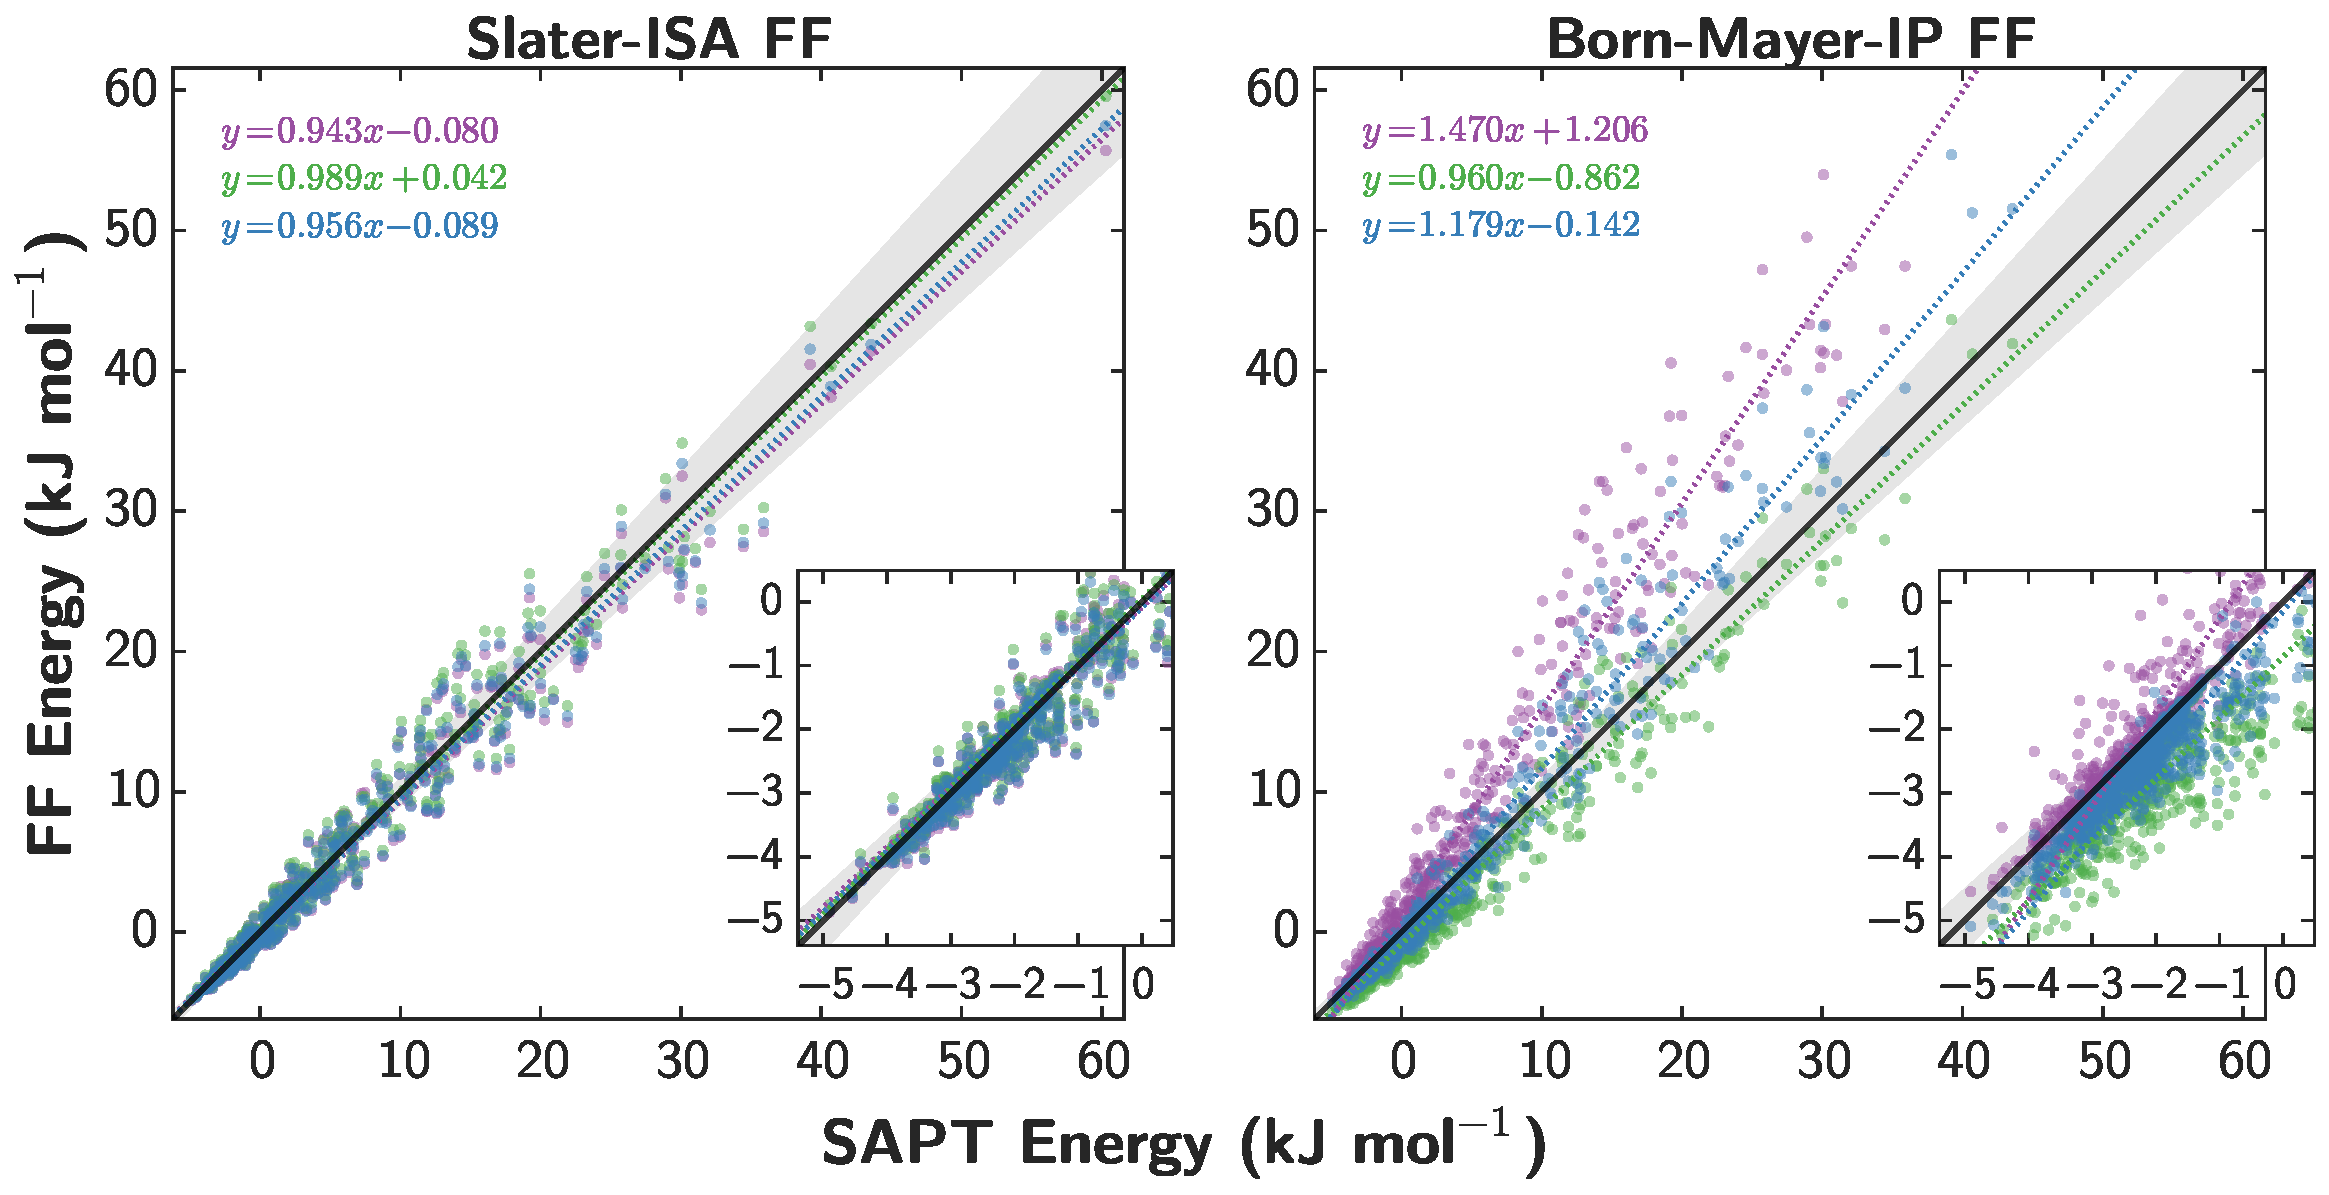
\includegraphics[width=0.9\textwidth]{isotropic/compare_ethane_ethane_scatter.pdf}
      \vfill
      \vfill
        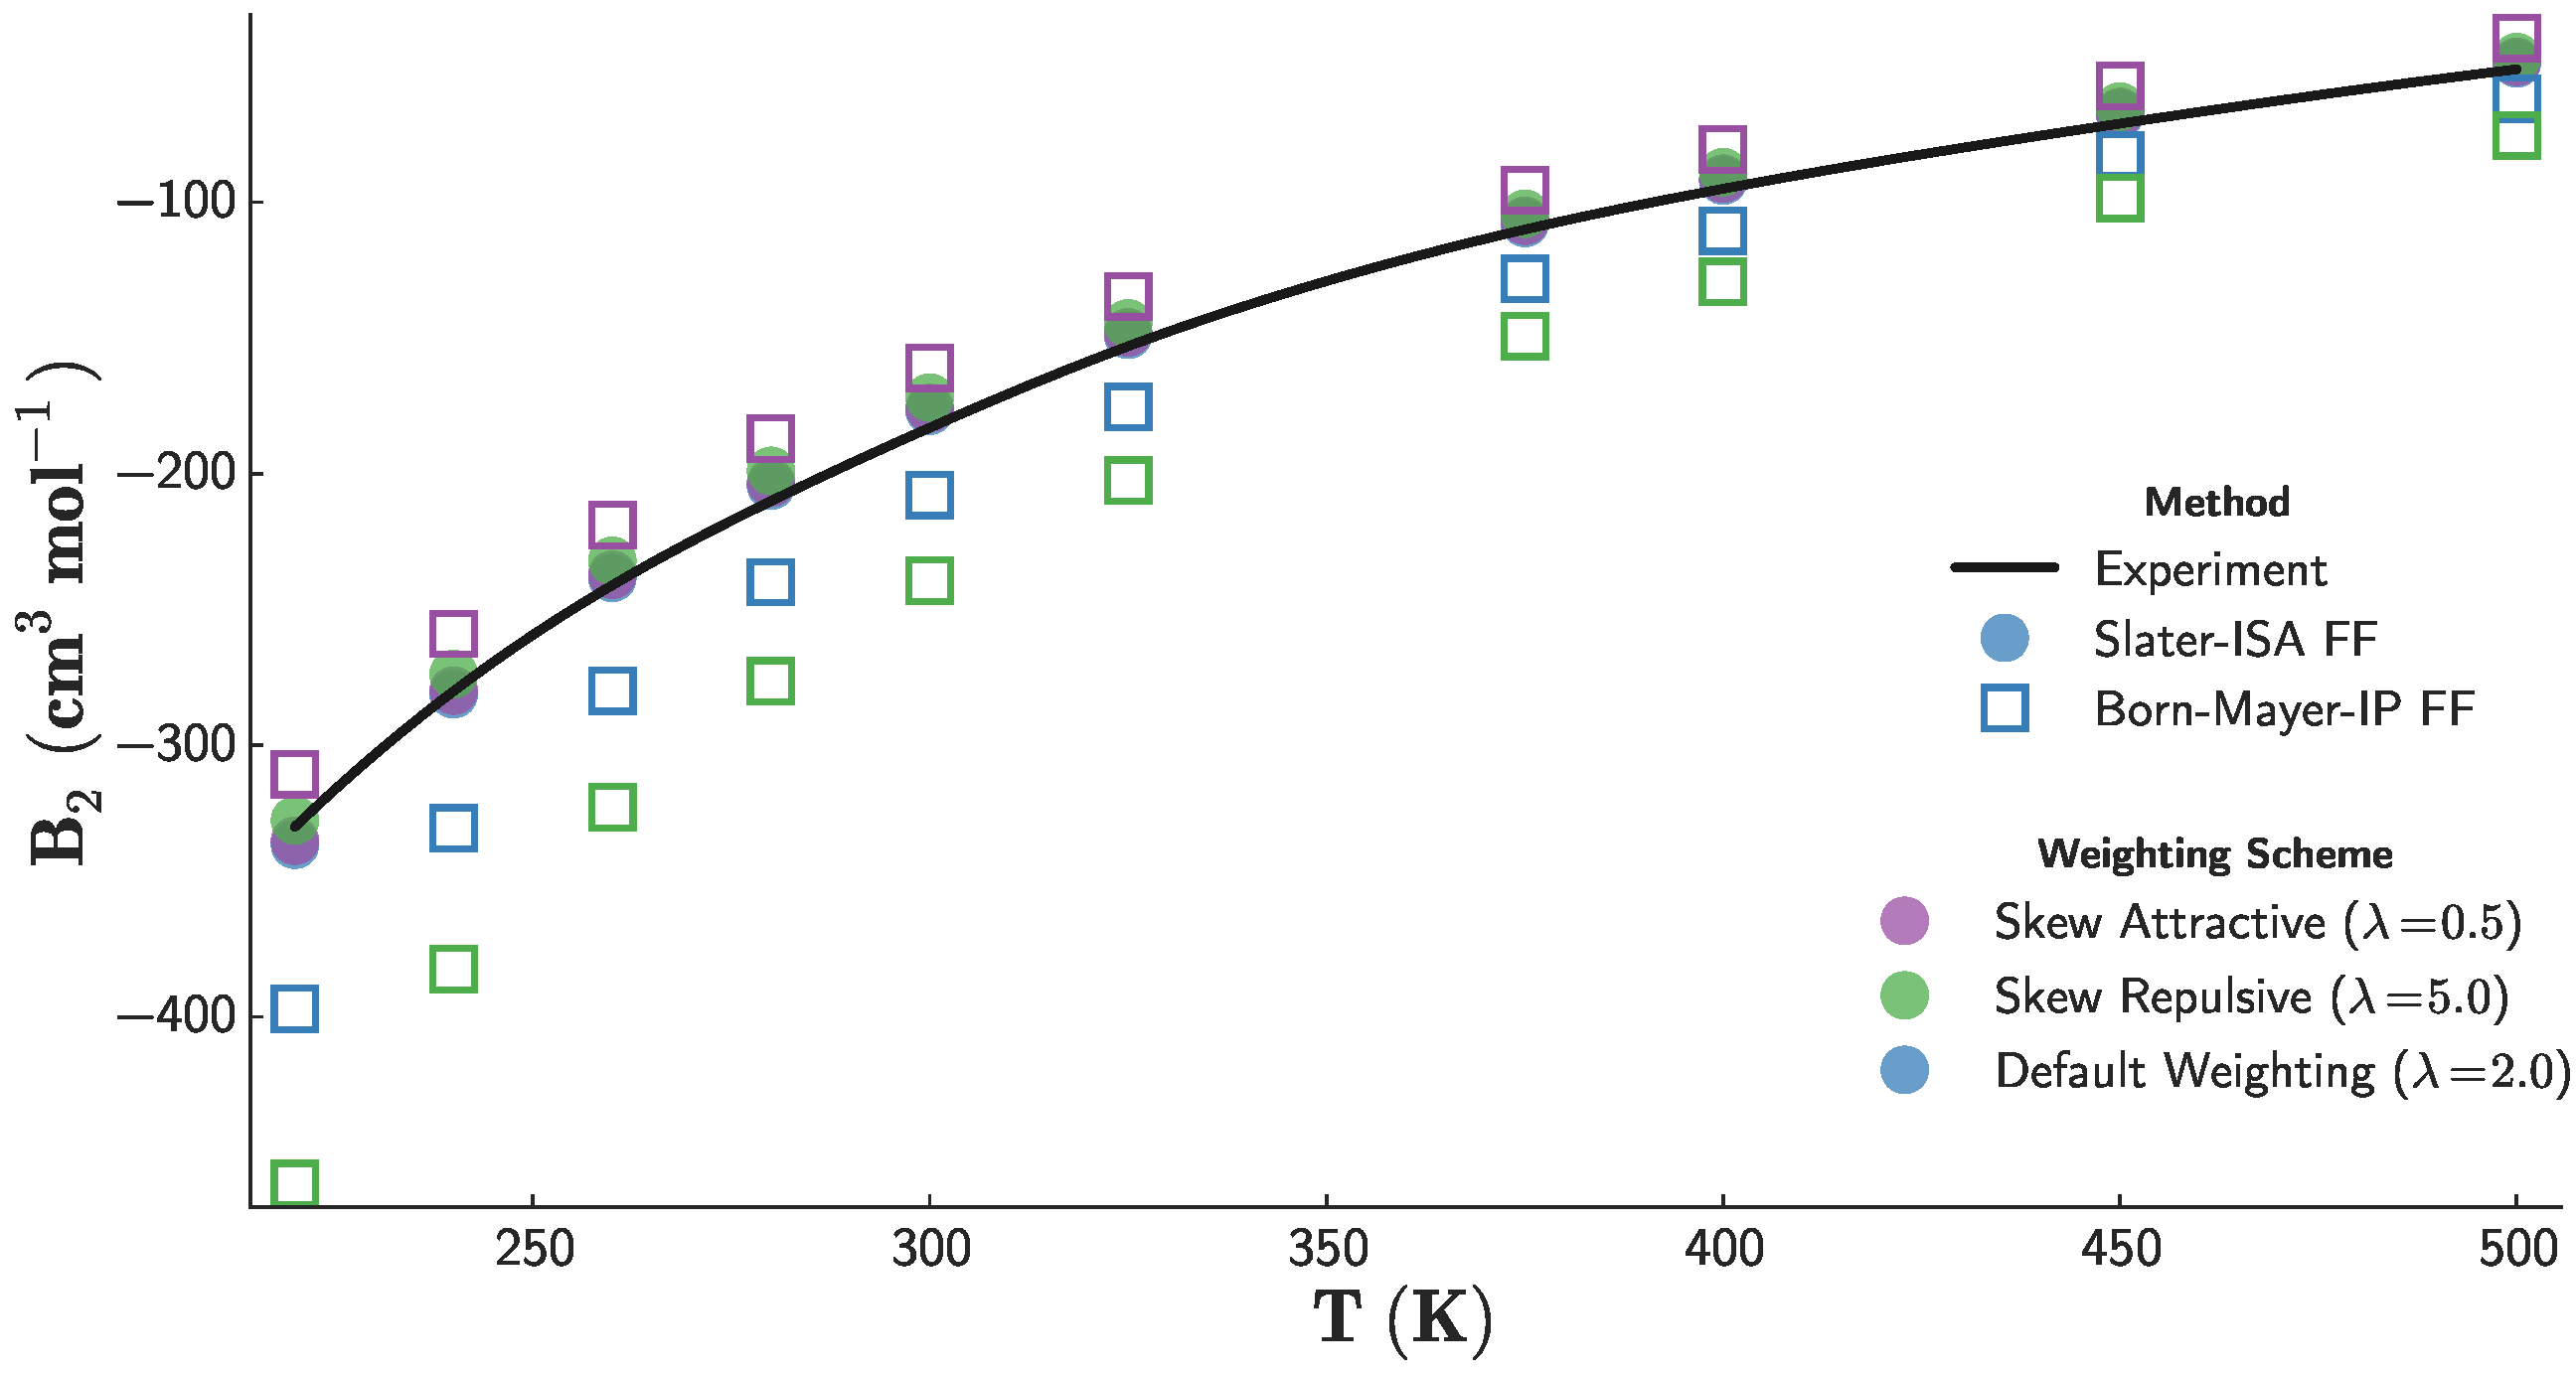
\includegraphics[width=0.9\textwidth]{isotropic/weighted_ethane_2nd_virial.pdf}
      \caption[foo]{
        Comparison of the \isaffold and the \saptff in terms of sensitivity to the
        weighting function employed in parameter optimization for the ethane
        dimer. Three weighting functions, $\lambda = 0.5$ (purple), $\lambda = 2.0$
        (blue), and $\lambda = 5.0$ (green) are shown, with higher $\lambda$ values
        indicating more weighting of repulsive configurations.
        
        (top) Total interaction energies for the \isaffold (left) and the \saptff (right)
        indicating the accuracy of each force field with respect to \saptpbeo benchmark
        energies.  The diagonal line (black) indicates perfect agreement between
        reference energies and each force field, while shaded grey areas represent
        points within $\pm 10\%$ agreement of the benchmark.  To guide the eye, a line
        of best fit (dotted line) has been computed for each force field and for each
        weighting function.
        
        (bottom) Computed 2$^\text{nd}$ virial coefficients for ethane. Data for
        the \isaffold and the \saptff are depicted using shaded circles and open squares,
        respectively; colors for the different weighting functions are as above.
        Experimental data from \citen{Dymond1980} (black line) is also shown.
        %ASK: Do we actually cite Dymond and Smith for this, since it's a compiled
        %work, or do I need to try and dig up the original experimentalist?
    }
    \label{fig:isotropic-ethane-weighting}

    \end{figure}
    %%%%%%%% Weighting Function Tests %%%%%%%

The \isaffold fits for the ethane dimer, on the other hand, are nearly completely
insensitive to the weighting function, leading to little intrinsic uncertainty
in the determination of parameters or in the computation of macroscopic
properties. Some other dimers, particularly those where
atomic anisotropy would be anticipated (e.g., water), exhibited slightly larger
sensitivity to the weighting function. Nevertheless, the
vast majority of dimers in the test set are qualitatively insensitive to the choice of
weighting function, and can be optimized with the default $\lambda = 2.0$
weighting function without yielding undue systematic error in the attractive
region of the potential, thus proving the enhanced robustness of the \isaffold
model relative to conventional force fields.

\end{subsection}
\begin{subsection}{Next-Generation Born-Mayer Models: \bmsisaff}

We hypothesize that the increased accuracy, transferability, and robustness of
the \isaffold is a direct result of its more physically-motivated functional form and
its use of ISA-derived atomic exponents that directly account for the influence
of the molecular environment. Nonetheless, we recognize that the standard
Born-Mayer functional form remains extremely common, both in simulation software and in
existing force fields. It is therefore fruitful to explore the extent to which the \bsisa
exponents themselves could be used in conjunction with a Born-Mayer functional
form. These results are shown in \cref{tab:isotropic-bmsisaff_rmse}.

%%%%%%%%%%%%%%%%%%%%% Average RMSE Table %%%%%%%%%%%%%%%%%%%%%%%%%%%%%%%%%%%
\begin{landscape}
\begin{table}
\footnotesize
\centering
\renewcommand\arraystretch{1.1}
\begin{tabular}{@{}rcccccccc@{}}
\hline
\toprule
& \phantom{ab} &
  \multicolumn{3}{c}{Dimer-Specific Fits} &
  \phantom{ab} &
  \multicolumn{3}{c}{Transferable Fits} \\
\cmidrule{3-5} \cmidrule{7-9}

Component & & \isaffold & Born-Mayer-ISA & Born-Mayer-sISA & & \isaffold & Born-Mayer-ISA & Born-Mayer-sISA  \\
     & & \multicolumn{1}{c}{(kJ mol$^{-1}$)} & \multicolumn{1}{c}{(kJ mol$^{-1}$)} &  \multicolumn{1}{c}{(kJ mol$^{-1}$)}
     & & \multicolumn{1}{c}{(kJ mol$^{-1}$)}& \multicolumn{1}{c}{(kJ mol$^{-1}$)} &  \multicolumn{1}{c}{(kJ mol$^{-1}$)} \\
\midrule
Exchange        & &    2.641 (0.686)   &  7.030 (1.203)     &  2.677 (0.686)  & &    2.718 (0.720)  &  6.968 (1.228)  & 2.764 (0.706) \\
Electrostatics  & &    1.087 (0.351)   &  1.406 (0.589)     &  1.083 (0.352)  & &    1.134 (0.351)  &  1.461 (0.598)  & 1.141 (0.352) \\
Induction       & &    0.251 (0.095)   &  0.229 (0.097)     &  0.250 (0.096)  & &    0.278 (0.101)  &  0.257 (0.101)  & 0.275 (0.101) \\
\dhf            & &    0.246 (0.068)   &  0.327 (0.120)     &  0.248 (0.068)  & &    0.274 (0.076)  &  0.353 (0.122)  & 0.274 (0.076) \\
Dispersion      & &    0.766 (0.317)   &  3.584 (0.890)     &  0.856 (0.336)  & &    0.766 (0.317)  &  3.584 (0.890)  & 0.856 (0.336) \\
\addlinespace                                                                                                           
\textbf{                                                                                                                    
Total Energy}   \\
\emph{RMSE}
                & &    1.701 (0.464)   &  4.934 (1.054)     &  1.751 (0.453)  & &    1.650 (0.456)  &  4.555 (1.035)  & 1.713 (0.446) \\
\emph{\mse}
                & &    0.216 (0.057)   &  1.127 (0.505)     &  0.258 (0.063)  & &    0.175 (0.051)  &  0.882 (0.516)  & 0.245 (0.057) \\
\bottomrule

\hline
\end{tabular}
\caption{
    Comparison of characteristic RMSE (as described in the main text) over the 91 dimer test
set for the 
    Born-Mayer-sISA approximation compared with other methods.
    For the total energy, both RMSE and absolute mean signed errors
    (MSE) have been shown.
    `Attractive' RMSE, representing the characteristic RMSE for
    the subset of points whose energies are net attractive ($\etot <
    0$), are shown in parentheses to the right of the total RMS
    errors; `attractive' \mse are likewise displayed for the total
    energy.
    \isaffold, Born-Mayer-ISA, and \bmsisaff are as described in the main text,
and the `Dimer-Specific' and `Transferable' fits are as described in
\cref{tab:isotropic-rmse}.
	}
\label{tab:isotropic-bmsisaff_rmse}
\end{table}
\normalsize
\end{landscape}
%%%%%%%%%%%%%%%%%%%%% Average RMSE Table %%%%%%%%%%%%%%%%%%%%%%%%%%%%%%%%%%%

As expected, direct insertion of the \bsisa exponents into the
Born-Mayer functional form (Born-Mayer-ISA) does not yield promising results.
Indeed, the Born-Mayer-ISA FF has significantly worse RMSE and \mse than
the \saptff. 
We reiterate that the $P = 1$ approximation from \cref{eq:isotropic-isaff_sr}, yielding the
conventional Born-Mayer form, is by itself a crude model.
Rather, it becomes necessary to accompany this approximation by a
corresponding exponent scale factor, $\xi$:
%
\begin{align}
\label{eq:isotropic-bmsisaff_bi}
B_i &= \xi \Bisa{i}.
\end{align}
%
Following literature precedent, 
\cite{Ihm1990, McDaniel2012}
we hypothesized that $\xi$ could be treated as a
universal constant. To test this conjecture, we computed reference density overlaps for a
variety of isolated atom pairs (details in the Supporting Information of
\citen{VanVleet2016}), and
fitted each of these overlaps to a Born-Mayer function of the form 
$S_{ij} \approx K_{ij}\exp(-\xi \Bisa{ij} \R)$, where $K_{ij} =
\frac{K}{B^{3}_{ij}}$ in line with \cref{eq:isotropic-isaff_aij}. To very good
approximation, both $K$ and $\xi$ can be treated as universal constants;
that is, neither $K$ nor $\xi$ is sensitive to the value of $\Bisa{}$.
However, fitted values of $K$ and $\xi$ do depend strongly on the range of \R values
used in the optimization, yielding estimates ranging from 0.74 to 0.88.

As an alternative, we optimized $\xi$ directly by minimizing RMSE
against the 91 dimer test set. Results from various choices
of $\xi$ can be found in the Supporting Information of \citen{VanVleet2016}.  In agreement
with prior literature and our `first-principles' analysis of overlaps, we find $\xi
= 0.84$ to be optimal for minimizing characteristic overall and attractive RMSE,
though in practice the errors are insensitive to $\xi \in [0.82,0.86]$.
We henceforth use $\xi=0.84$ and refer to to this force field methodology
(Born-Mayer functional form, ISA-derived exponents with
scale factor $\xi=0.84$) as the \bmsisaff. 
Parameters and homo-monomeric fits for the \bmsisaff
can be found in the Supporting Information of \citen{VanVleet2016} and in
\cref{sec:isotropic-homomonomeric_fits}.
 
From \cref{tab:isotropic-bmsisaff_rmse} we see that the \bmsisaff is comparable in
quality to our original \isaffold methodology. 
For all attractive configurations, the \bmsisaff is equally
accurate and transferable (\cref{tab:isotropic-bmsisaff_rmse}). Furthermore, as shown in
\cref{tab:isotropic-rmsd-weightings}, \bmsisaff displays similar parameter robustness
to \isaffold. These results suggest that many of the advantages of the \isaffold
procedure can be captured simply by using the (scaled) ISA exponents.
Note, however, that the optimal scale factor likely exhibits some system dependence,
and furthermore that the enhanced Slater functional form may be important
where an accurate description of highly repulsive configurations is crucial.

We also examined the \isaffold and the \bmsisaff against force
fields where $B_i$ values were instead treated as soft constraints, rather than fixed parameters.
Using entirely unconstrained exponents yields unphysical parameters and a 
severe degradation in force field transferability. Using exponents from the \isaffold and
the \bmsisaff as Bayesian priors (in the sense used in
\citens{Misquitta2015a,Misquitta2015b}), 
we generated two new force fields with optimized exponents, denoted Slater-OPT and Born-Mayer-OPT,
respectively. Characteristic RMSE and \mse for these force fields can be found
in the Supporting Information of \citen{VanVleet2016}.
We find that both methods yield only very minimal improvement, suggesting that the
first-principles ISA exponents are already nearly optimal. Comparing the Born-Mayer-OPT
exponents to those from Slater-ISA, we find a nearly identical average scale factor
of $\gamma = 0.83 \pm 0.07$.  Given that these optimal exponents can now be generated
directly from first principles calculations of the molecular densities via the \bsisa 
approach of \citeauthor{Misquitta2014}, we anticipate that the \bsisa densities and
resulting ISA exponents will be extremely useful in next-generation force field
development in order to greatly simplify force field parameterization.

\end{subsection}
